% Chapter Template

\chapter{Domain-invariant features for mechanism of action prediction in a multi-cell-line drug screen} % Main chapter title

\label{Chapter3} % Change X to a consecutive number; for referencing this chapter elsewhere, use \ref{ChapterX}
\chaptermark{Domain-invariant features}

%\lhead{Chapter 2. \emph{Supervised Sequence Learning}} % Change X to a consecutive number; this is for the header on each page - perhaps a shortened title

\textbf{Summary}: \emph{High Content Screening is an important tool in drug discovery and characterisation. Often, high content drug screens are performed on one single cell line. Yet, a single cell line cannot be thought of as a perfect disease model. Many diseases feature an important molecular heterogeneity. Consequently, a drug may be effective against one molecular subtype of a disease, but less so against another. To characterise drugs with respect to their effect not only on one cell line but on a panel of cell lines is therefore a promising strategy to streamline the drug discovery process. The contribution of this paper is twofold. First, we investigate whether we can predict drug mechanism of action (MOA) at the molecular level without optimisation of the MOA classes to the screen specificities. To this end, we benchmark a set of algorithms within a conventional pipeline, and evaluate their MOA prediction performance according to a statistically rigorous framework. Second, we extend this conventional pipeline to the simultaneous analysis of multiple cell lines, each manifesting potentially different morphological baselines. For this, we propose multitask autoencoders, including a domain-adaptive model used to construct domain-invariant feature representations across cell lines. We apply these methods to a pilot screen of two triple negative breast cancer cell lines as models for two different molecular subtypes of the disease.}

\textbf{R\'esum\'e}: \emph{Cette chapitre...}

% High Content Screening
\section{Introduction}
% High Content Screening
High content screening (HCS) is a powerful tool for identifying potential drugs effective against a particular disease. A high content drug screen corresponds to a series of imaging experiments under controlled conditions, where a cell line representative of some disease is exposed to a large panel of drugs. For each drug, one obtains a set of images informative of its phenotypic effect and hence on the biological pathways undergoing perturbation. Various advances in microscopy automation and image analysis have pushed HCS to the early \emph{hit-to-lead} stages of the drug discovery process \cite{haney2006high}.

% MOA
% --> MOA can be at different levels 
% --> HCS is optimized w.r.t particular pathways.
% --> MOA is difficult in general for this reason (even though it may be easy in specific cases.)
The discovery of new drugs may be guided by a reference set of drugs of known mechanism of action (MOA). The MOA of a drug is the particular cellular pathway it perturbs to achieve its effect. Through application of image analysis, one may attempt to infer the MOA of an unknown drug from HCS image data. Note that MOA can be defined at different levels and with different degrees of specificity: MOA might concern the exact protein that is targeted (e.g. AURKA inhibition), or a specific effect on cellular components (e.g. stabilisation of microtubuli) or perturbation of a more general cellular pathway (e.g. DNA repair). HCS is usually optimised with respect to particular pathways by the choice of the fluorescent markers and readouts {\cite{pepperkok2006}}. {Consequently, MOA prediction might be reasonably straightforward if MOA classes are chosen in accordance with the phenotypic readout \cite{ljosa2013comparison}}, but it is challenging in general, in particular if we aim at predicting specific MOAs the assay has not been optimised for.

%Of note, the exact meaning of MOA can be very different from study to study, 


% Such an effect manifests as a set of aberrant cellular morphologies with respect to a negative control population. Through application of image analysis, one may attempt to infer the MOA of an unknown drug from HCS image data. 
% A conventional approach is to produce for each drug a \emph{phenotypic profile}, that is, a vector of features characterising a drug effect on a cell population. The MOA of an unknown drug can then be predicted through comparison of its profile with those of the known reference drugs. 

% Why multiple cell lines?
A second difficulty concerns the cellular model that is used. As a proxy for diseased cells, a cell line cannot be thought of as a perfect model. Many diseases feature a significant molecular heterogeneity. Consequently, a drug may be effective against one molecular subtype of a disease, but less so against another. Furthermore, immortalised cell lines may diverge over time due to genetic drift. For example, HeLa, the quintessential cell line, is famously the cause of great scientific confusion {due to difficulties in cell line identification \cite{horbach2017ghosts} and significant molecular and phenotypic variability \cite{liu2019multi}}. To characterise drugs with respect to their effect not only on one cell line but on a consensus of several is therefore a promising strategy to streamline the drug discovery process. Nevertheless, this is not an easy task in morphological screening, as different cell lines usually have distinct archetypal morphologies even prior to perturbation. It is therefore conceptually difficult to characterise and compare drug effects across cell lines.

% Contribution of the paper. 
The contribution of this paper is twofold. First, we investigate whether we can predict MOA at the molecular level without optimisation of the MOA classes to the screen specificities. To this end, we benchmark a set of algorithms within a conventional pipeline, and evaluate their MOA prediction performance according to a statistically rigorous framework.

Second, we extend this conventional pipeline to the simultaneous analysis of multiple cell lines, each with potentially different morphological baselines. For this, we propose multitask autoencoders, including an adaptive model used to construct domain-invariant feature representations across cell lines. We apply these methods to a pilot screen of two triple negative breast cancer (TNBC) cell lines as models for two different molecular subtypes of the disease.

% Organization of the paper
In Section \ref{sec:data}, we describe our data set. In Section \ref{sec:methods} we formalise a range of profiling approaches from the literature according to four key properties, and extend this to a multi-cell-line analysis. In Section \ref{sec:results} we illustrate the benefit of multi-task models for our dataset through extensive cross-validation and provide an exploratory analysis of differential drug effects between the two cell lines. In Section \ref{sec:discussion} we discuss our methods and the obtained results.

%\enlargethispage{12pt}


% Title page, Structured Abstract, Introduction, System and methods, Algorithm, Implementation, Discussion, References

\section{Data}
\label{sec:data}
We acquired image data for two triple-negative breast cancer (TNBC) cell lines, MDA-MB-231 and MDA-MB-468 (hereafter MDA231 and MDA468), thus constituting a multi-cell-line drug screen\footnote{The full image set for this study is available at \texttt{https://zenodo.org/record/2677923}}. {MDA231 (TP53, KRAS, BRAF) and MDA468 (TP53-PTEN) were both established from a pleural effusion of two different patients with triple negative metastatic breast carcinoma. Using transcriptomic and genomic data, we have recently shown that MDA468 clustered in a breast cancer specific subgroup but MDA231, one of the most used breast cancer cell lines, clustered in a mixed subgroup with cancer cell lines of very different origins, such as ovarian, urinary and kidney \cite{Sadacca2017}.}

Both of our cell lines were subjected to the same inventory of drugs on separate 384-well microtiter plates (microplates): 36 wells contained the negative control dimethyl sulfoxide (DMSO); two the positive controls (Olaparib, Cisplatine); 166 the test compounds; and 184 empty. For each well of our two microplates, images were taken in four non-overlapping fields of view (fields), with three multiplexed fluorescent channels: (1) DAPI (cell nuclei) (2) Cyanine 3 (Cy3, $\gamma$H2AX to mark DNA double-strand breaks), and (3) Cyanine 5 (Cy5; tubulin marker). Together, these fluorescent channels paint a rich, composite picture of the cell populations.

The drugs comprise of a set of panels of kinase, protease and phosphatase inhibitors and can be categorised into 70 MOA classes of varying sizes, according to their targets. For our experiments, we take the 8 MOA classes having at least five member drugs. These are CDK inhibitors, cysteine protease inhibitors, EGF receptor kinase inhibitors, MMP inhibitors, DMSO (negative control), PKC inhibitors, protein tyrosine phosphatase inhibitors, and tyrosine kinase inhibitors.

In comparison with other datasets, \cite{adams2006compound} used 51 drugs in 13 MOA categories, \cite{slack2008characterizing} used 35 drugs in six MOA categories, and the widely studied Broad Institute Benchmark Collection 21 (BBBC21v2) \cite{ljosa2012annotated} -- used, for example, in \cite{kandaswamy2016high} and \cite{godinez2017multi} -- consists of 39 drugs in 13 categories. The key difference is that our own MOA classes were not selected \emph{a posteriori} to reflect visually different phenotypes, mounting a greater bioinformatic challenge than the standard benchmark datasets, where even a simple model can be extremely effective. For example, \cite{singh2014pipeline} achieved $90\%$ accuracy with element-wise averaging of hand-crafted features after a simple luminosity correction.

%The particular choice of drugs, chosen for their cytotoxic properties, made for a challenging classification problem. This prompted a comparison of the commonly used approaches to phenotypic profiling from the literature, along with innovations and extensions for multi cell line analysis. \cite{ljosa2013comparison} compared five such approaches on what has become a standard benchmark dataset. Since this study, the deep learning revolution has entered into high content analysis, and we aim here to include such techniques in the comparison. In Section \ref{sec:methods} we characterise a range of profiling approaches from the literature according to four key properties, and extend these to a multi cell line analysis in novel ways. In Section \ref{sec:results} we establish the optimal profiling approach for our dataset through extensive cross validation. This then facilitates an exploratory anaylsis in Section \ref{sec:discussion} into the differential drug effects between the two cell lines.

\section{Methods}
\label{sec:methods}

\begin{figure}
\centering

\tikzset{every picture/.style={line width=0.75pt}} %set default line width to 0.75pt        

\begin{tikzpicture}[x=0.75pt,y=0.75pt,yscale=-1.5,xscale=1.5]
%uncomment if require: \path (0,436); %set diagram left start at 0, and has height of 436

%Pentagon Arrow [id:dp6130111799740185] 
\draw   (104,157) -- (110,157) -- (114,162) -- (110,167) -- (104,167) -- cycle ;
%Straight Lines [id:da06258955071050465] 
\draw    (214,142) -- (244,152) ;


%Straight Lines [id:da5937674565797327] 
\draw    (214,142) -- (244,172) ;


%Straight Lines [id:da2372852336366117] 
\draw    (214,152) -- (244,152) ;


%Straight Lines [id:da21758067008263982] 
\draw    (214,152) -- (244,172) ;


%Straight Lines [id:da16740793182069647] 
\draw    (214,142) -- (244,162) ;


%Straight Lines [id:da8627075277726398] 
\draw    (214,152) -- (244,162) ;


%Straight Lines [id:da21621905245992268] 
\draw    (214,162) -- (244,152) ;


%Straight Lines [id:da5980502763438268] 
\draw    (214,162) -- (244,162) ;


%Straight Lines [id:da21374798311805465] 
\draw    (214,162) -- (244,172) ;


%Straight Lines [id:da6958213914747777] 
\draw    (214,172) -- (244,152) ;


%Straight Lines [id:da3100913913415474] 
\draw    (214,172) -- (244,162) ;


%Straight Lines [id:da9769993626007268] 
\draw    (214,172) -- (244,172) ;


%Straight Lines [id:da549211858708586] 
\draw    (214,182) -- (244,152) ;


%Straight Lines [id:da735220903873294] 
\draw    (214,182) -- (244,162) ;


%Straight Lines [id:da16587942119765675] 
\draw    (214,182) -- (244,172) ;


%Shape: Circle [id:dp45757735000409094] 
\draw   (204,142) .. controls (204,139.24) and (206.24,137) .. (209,137) .. controls (211.76,137) and (214,139.24) .. (214,142) .. controls (214,144.76) and (211.76,147) .. (209,147) .. controls (206.24,147) and (204,144.76) .. (204,142) -- cycle ;
%Shape: Circle [id:dp7331962778010591] 
\draw   (214,182) .. controls (214,179.24) and (211.76,177) .. (209,177) .. controls (206.24,177) and (204,179.24) .. (204,182) .. controls (204,184.76) and (206.24,187) .. (209,187) .. controls (211.76,187) and (214,184.76) .. (214,182) -- cycle ;
%Shape: Circle [id:dp2501248555900335] 
\draw   (214,172) .. controls (214,169.24) and (211.76,167) .. (209,167) .. controls (206.24,167) and (204,169.24) .. (204,172) .. controls (204,174.76) and (206.24,177) .. (209,177) .. controls (211.76,177) and (214,174.76) .. (214,172) -- cycle ;
%Shape: Circle [id:dp8461118047726299] 
\draw   (214,152) .. controls (214,149.24) and (211.76,147) .. (209,147) .. controls (206.24,147) and (204,149.24) .. (204,152) .. controls (204,154.76) and (206.24,157) .. (209,157) .. controls (211.76,157) and (214,154.76) .. (214,152) -- cycle ;
%Shape: Circle [id:dp9802553651979097] 
\draw   (214,162) .. controls (214,159.24) and (211.76,157) .. (209,157) .. controls (206.24,157) and (204,159.24) .. (204,162) .. controls (204,164.76) and (206.24,167) .. (209,167) .. controls (211.76,167) and (214,164.76) .. (214,162) -- cycle ;
%Shape: Circle [id:dp8350886089645121] 
\draw   (244,152) .. controls (244,149.24) and (246.24,147) .. (249,147) .. controls (251.76,147) and (254,149.24) .. (254,152) .. controls (254,154.76) and (251.76,157) .. (249,157) .. controls (246.24,157) and (244,154.76) .. (244,152) -- cycle ;
%Shape: Circle [id:dp8566895153060261] 
\draw   (254,162) .. controls (254,159.24) and (251.76,157) .. (249,157) .. controls (246.24,157) and (244,159.24) .. (244,162) .. controls (244,164.76) and (246.24,167) .. (249,167) .. controls (251.76,167) and (254,164.76) .. (254,162) -- cycle ;
%Shape: Circle [id:dp9730393642848857] 
\draw   (254,172) .. controls (254,169.24) and (251.76,167) .. (249,167) .. controls (246.24,167) and (244,169.24) .. (244,172) .. controls (244,174.76) and (246.24,177) .. (249,177) .. controls (251.76,177) and (254,174.76) .. (254,172) -- cycle ;

%Shape: Rectangle [id:dp01893061250967598] 
\draw   (124,137) -- (134,137) -- (134,147) -- (124,147) -- cycle ;
%Shape: Rectangle [id:dp9999227766849469] 
\draw   (134,137) -- (144,137) -- (144,147) -- (134,147) -- cycle ;
%Shape: Rectangle [id:dp5617645410371781] 
\draw  [fill={rgb, 255:red, 169; green, 90; blue, 161 }  ,fill opacity=1 ] (144,137) -- (154,137) -- (154,147) -- (144,147) -- cycle ;
%Shape: Rectangle [id:dp3035053657099249] 
\draw   (154,137) -- (164,137) -- (164,147) -- (154,147) -- cycle ;
%Shape: Rectangle [id:dp8541883561222736] 
\draw   (164,137) -- (174,137) -- (174,147) -- (164,147) -- cycle ;
%Shape: Rectangle [id:dp9811252901850964] 
\draw  [fill={rgb, 255:red, 133; green, 192; blue, 249 }  ,fill opacity=1 ] (124,147) -- (134,147) -- (134,157) -- (124,157) -- cycle ;
%Shape: Rectangle [id:dp052261541447719884] 
\draw   (134,147) -- (144,147) -- (144,157) -- (134,157) -- cycle ;
%Shape: Rectangle [id:dp46612464110376217] 
\draw   (144,147) -- (154,147) -- (154,157) -- (144,157) -- cycle ;
%Shape: Rectangle [id:dp8684616287136228] 
\draw   (154,147) -- (164,147) -- (164,157) -- (154,157) -- cycle ;
%Shape: Rectangle [id:dp731115381112905] 
\draw   (164,147) -- (174,147) -- (174,157) -- (164,157) -- cycle ;
%Shape: Rectangle [id:dp11035542720674363] 
\draw   (124,157) -- (134,157) -- (134,167) -- (124,167) -- cycle ;
%Shape: Rectangle [id:dp7130234560992348] 
\draw   (134,157) -- (144,157) -- (144,167) -- (134,167) -- cycle ;
%Shape: Rectangle [id:dp744392771028909] 
\draw   (144,157) -- (154,157) -- (154,167) -- (144,167) -- cycle ;
%Shape: Rectangle [id:dp2652512133402899] 
\draw  [fill={rgb, 255:red, 245; green, 121; blue, 58 }  ,fill opacity=1 ] (154,157) -- (164,157) -- (164,167) -- (154,167) -- cycle ;
%Shape: Rectangle [id:dp789626378851182] 
\draw   (164,157) -- (174,157) -- (174,167) -- (164,167) -- cycle ;
%Shape: Rectangle [id:dp6507666674673268] 
\draw  [fill={rgb, 255:red, 245; green, 121; blue, 58 }  ,fill opacity=1 ] (124,167) -- (134,167) -- (134,177) -- (124,177) -- cycle ;
%Shape: Rectangle [id:dp7794048817725451] 
\draw   (134,167) -- (144,167) -- (144,177) -- (134,177) -- cycle ;
%Shape: Rectangle [id:dp7170628281281102] 
\draw   (144,167) -- (154,167) -- (154,177) -- (144,177) -- cycle ;
%Shape: Rectangle [id:dp9654720754525126] 
\draw   (154,167) -- (164,167) -- (164,177) -- (154,177) -- cycle ;
%Shape: Rectangle [id:dp2644320789753808] 
\draw   (164,167) -- (174,167) -- (174,177) -- (164,177) -- cycle ;
%Shape: Rectangle [id:dp9474374800359919] 
\draw   (124,177) -- (134,177) -- (134,187) -- (124,187) -- cycle ;
%Shape: Rectangle [id:dp27886448200839375] 
\draw   (134,177) -- (144,177) -- (144,187) -- (134,187) -- cycle ;
%Shape: Rectangle [id:dp21216168672979663] 
\draw   (144,177) -- (154,177) -- (154,187) -- (144,187) -- cycle ;
%Shape: Rectangle [id:dp1866508286696681] 
\draw   (154,177) -- (164,177) -- (164,187) -- (154,187) -- cycle ;
%Shape: Rectangle [id:dp7447818762358708] 
\draw  [fill={rgb, 255:red, 133; green, 192; blue, 249 }  ,fill opacity=1 ] (164,177) -- (174,177) -- (174,187) -- (164,187) -- cycle ;
%Pentagon Arrow [id:dp6664158537123742] 
\draw   (184,157) -- (190,157) -- (194,162) -- (190,167) -- (184,167) -- cycle ;
%Pentagon Arrow [id:dp5743225440952848] 
\draw   (264,157) -- (270,157) -- (274,162) -- (270,167) -- (264,167) -- cycle ;
%Image [id:dp1770251862166521] 
%\draw (69,162) node  {\includegraphics[width=37.5pt,height=37.5pt]{img/overlay.png}};
\draw (69,162) node  {\includegraphics[width=56.25pt,height=56.25pt]{img/overlay.png}};
%Shape: Rectangle [id:dp2951489537408193] 
\draw   (124,137) -- (174,137) -- (174,187) -- (124,187) -- cycle ;
%Straight Lines [id:da08376425563228318] 
\draw    (44,121.5) -- (189,121.5) ;


%Straight Lines [id:da1606287579095167] 
\draw    (189,121.5) -- (334,121.5) ;


%Straight Lines [id:da5725307105818378] 
\draw    (189,121.5) -- (189,116.5) ;


%Straight Lines [id:da5865138131900499] 
\draw    (44,126.5) -- (44,121.5) ;


%Straight Lines [id:da8216798303337918] 
\draw    (334,126.5) -- (334,121.5) ;


%Pentagon Arrow [id:dp8103808140917655] 
\draw   (144,51.5) -- (150,51.5) -- (154,56.5) -- (150,61.5) -- (144,61.5) -- cycle ;
%Pentagon Arrow [id:dp8808569829821885] 
\draw   (224,51.5) -- (230,51.5) -- (234,56.5) -- (230,61.5) -- (224,61.5) -- cycle ;
%Image [id:dp09602617376087497] 
%\draw (109,56.5) node  {\includegraphics[width=37.5pt,height=37.5pt]{img/original.png}};
\draw (109,56.5) node  {\includegraphics[width=56.25pt,height=56.25pt]{img/original.png}};
%Shape: Circle [id:dp29625759093060444] 
\draw  [color={rgb, 255:red, 0; green, 0; blue, 0 }  ,draw opacity=1 ][fill={rgb, 255:red, 155; green, 155; blue, 155 }  ,fill opacity=1 ] (244,76.5) .. controls (244,73.74) and (246.24,71.5) .. (249,71.5) .. controls (251.76,71.5) and (254,73.74) .. (254,76.5) .. controls (254,79.26) and (251.76,81.5) .. (249,81.5) .. controls (246.24,81.5) and (244,79.26) .. (244,76.5) -- cycle ;
%Straight Lines [id:da1340161587824641] 
\draw  [dash pattern={on 4.5pt off 4.5pt}]  (244,31.5) -- (294,81.5) ;


%Shape: Circle [id:dp795205502785717] 
\draw  [color={rgb, 255:red, 0; green, 0; blue, 0 }  ,draw opacity=1 ][fill={rgb, 255:red, 155; green, 155; blue, 155 }  ,fill opacity=1 ] (254,66.5) .. controls (254,63.74) and (256.24,61.5) .. (259,61.5) .. controls (261.76,61.5) and (264,63.74) .. (264,66.5) .. controls (264,69.26) and (261.76,71.5) .. (259,71.5) .. controls (256.24,71.5) and (254,69.26) .. (254,66.5) -- cycle ;
%Shape: Circle [id:dp5861156631141803] 
\draw  [color={rgb, 255:red, 0; green, 0; blue, 0 }  ,draw opacity=1 ][fill={rgb, 255:red, 155; green, 155; blue, 155 }  ,fill opacity=1 ] (264,76.5) .. controls (264,73.74) and (266.24,71.5) .. (269,71.5) .. controls (271.76,71.5) and (274,73.74) .. (274,76.5) .. controls (274,79.26) and (271.76,81.5) .. (269,81.5) .. controls (266.24,81.5) and (264,79.26) .. (264,76.5) -- cycle ;
%Shape: Triangle [id:dp5263640774818461] 
\draw  [fill={rgb, 255:red, 155; green, 155; blue, 155 }  ,fill opacity=1 ] (269,31.5) -- (274,41.5) -- (264,41.5) -- cycle ;
%Shape: Triangle [id:dp48426466652695976] 
\draw  [fill={rgb, 255:red, 155; green, 155; blue, 155 }  ,fill opacity=1 ] (289,31.5) -- (294,41.5) -- (284,41.5) -- cycle ;
%Shape: Triangle [id:dp04587248999521798] 
\draw  [fill={rgb, 255:red, 155; green, 155; blue, 155 }  ,fill opacity=1 ] (279,41.5) -- (284,51.5) -- (274,51.5) -- cycle ;
%Shape: Rectangle [id:dp9433051376358494] 
\draw  [fill={rgb, 255:red, 245; green, 121; blue, 58 }  ,fill opacity=1 ] (164,51.5) -- (174,51.5) -- (174,61.5) -- (164,61.5) -- cycle ;
%Shape: Rectangle [id:dp5993980236375129] 
\draw  [fill={rgb, 255:red, 133; green, 192; blue, 249 }  ,fill opacity=1 ] (184,51.5) -- (194,51.5) -- (194,61.5) -- (184,61.5) -- cycle ;
%Shape: Rectangle [id:dp5967537610073326] 
\draw  [fill={rgb, 255:red, 169; green, 90; blue, 161 }  ,fill opacity=1 ] (204,51.5) -- (214,51.5) -- (214,61.5) -- (204,61.5) -- cycle ;
%Shape: Rectangle [id:dp16177370225507393] 
\draw   (174,51.5) -- (184,51.5) -- (184,61.5) -- (174,61.5) -- cycle ;
%Shape: Rectangle [id:dp4265637049532277] 
\draw   (194,51.5) -- (204,51.5) -- (204,61.5) -- (194,61.5) -- cycle ;

% Text Node
\draw (309,162) node [scale=7.5]  {$\Sigma $};
% Text Node
\draw (69,202.75) node [scale=0.7] [align=left] {Measurement unit};
% Text Node
\draw (149.5,203.5) node [scale=0.7] [align=left] {Feature representation};
% Text Node
\draw (229,203.5) node [scale=0.7] [align=left] {Dimensionality reduction};
% Text Node
\draw (309.5,203.5) node [scale=0.7] [align=left] {Aggregation strategy};
% Text Node
\draw (110,100) node [scale=0.7] [align=left] {Input image};
% Text Node
\draw (190,100) node [scale=0.7] [align=left] {Phenotypic profile};
% Text Node
\draw (269,100) node [scale=0.7] [align=left] {MOA prediction};

\end{tikzpicture}

\caption{MOA prediction is performed on an image via a phenotypic profile. The development of such a profile spans four ordered stages. Each stage may be accomplished by a variety of algorithms, the combination of which define a unique pipeline. Some stages may be omitted in certain pipelines, or subsumed to a common framework.}
\label{fig:profiling}
\end{figure}

This section describes the approaches for phenotypic profiling we have benchmarked. We embed these descriptions in a formalised overview of phenotypic profiling strategies to motivate the different setups. In Section \ref{subsec:multi_cell_line_analysis} we describe methods for a joint analysis of multiple cell lines.

\subsection{MOA prediction}
\label{subsec:moa_prediction}

Drugs are assigned a class based on their \emph{mechanism of action} (MOA), the cellular pathway perturbed by the drug, as depicted in Figure \ref{fig:profiling}. Given a set of drug profiles annotated with MOA classes, we can simulate reference and discovery drug sets in a \emph{leave-one-compound-out} cross-validation (LOCOCV) scheme. At each fold of the cross-validation, we hold out a drug and predict its MOA class using a classifier trained on the remaining ``reference'' drugs. The prediction is made as the nearest neighbour (1-NN) in cosine distance between drug profiles, $d(\mathbf{p}, \mathbf{p}') = 1 - \cos\theta_{\mathbf{p}, \mathbf{p}'}$. This was proposed in \cite{ljosa2013comparison} as an equitable way of comparing profiling algorithms. We settle for this lightweight approach as our focus here is on the discriminative power of the profiles.

Note that kNN on Euclidean distance for normalised data,

\begin{align}d_E(\mathbf{u}, \mathbf{v}) &= ||\mathbf{u} - \mathbf{v}||_2 \notag \\
&= \sqrt{\mathbf{u}^T\mathbf{v} - 2\mathbf{u}^T\mathbf{v} + \mathbf{v}^T\mathbf{v}} \notag \\
&= \sqrt{2 - 2\mathbf{u}^T\mathbf{v}} \notag \\
&= \sqrt{2d_{C}(\mathbf{u}, \mathbf{v})} \notag
\end{align}

where $d_{C}(\mathbf{u}, \mathbf{v})$ is the cosine distance between $\mathbf{u}$ and $\mathbf{v}$.

This is similar to a kernelised nearest centroids classifier, where the centroid is instead calculated in Euclidean space.

\begin{figure}
\centering
\includegraphics[width=\textwidth]{img/clustermap.pdf}
\label{fig:clustermap}
\end{figure}

\subsection{Phenotypic profiling}

The conventional approach to HCS analysis is a multi-stage pipeline, consisting of a sequence of modules of image and statistical analysis, including cell segmentation and hand-crafted feature extraction {\cite{Caicedo2017}}. The aim is to ascribe a phenotypic profile to each cell population to serve as the basis of comparison between drugs. Each profile will take the form of a vector $\mathbf{p} \in \mathbb{R}^D$ of some dimensionality $D$ and is constructed according to four ordered methodological stages: measurement unit, feature representation, dimensionality reduction, and aggregation strategy (Figure \ref{fig:profiling}). Certain properties may be omitted by some approaches, or subsumed to a common framework, such as a neural network, that may perform each task simultaneously \cite{kraus2016classifying,godinez2017multi}. In the following sections we detail each property in turn, providing references to the relevant literature and describing the concrete setup that was retained for the benchmarking.

%For example, one could first create a ground truth by annotating some sample cells according to an ontology of phenotypic forms (cell cycle phase, apoptosis, aberrant morphologies), and train a classifier to annotate the rest of the cell population \cite{neumann2010phenotypic}. There are two main drawbacks to this: the manual effort of creating the ground truth, and the difficulty in choosing a suitable ontology, in particular in cases where easily differentiated phenotypes are elusive. To preserve the automatic aspect of the pipeline, we focus primarily on approaches where this in-depth prior knowledge is not required.

\subsubsection{Measurement unit}
\label{subsubsec:unit}

The most common measurement unit is the cell itself, constituting a \emph{per-cell} analysis. This entails an initial segmentation of the cells (their nuclei and other organelles). We segmented cell nuclei on the DAPI channel by subtracting a background image formed with a mean filter, before clipping to zero. Touching nuclei were further separated by applying the watershed transform on the inverse distance map of the foreground image. The cytoplasm was segmented from the microtubule channel (Cy5) following \cite{jones2005voronoi}. 

Alternatively, one might analyse the image field directly in a \emph{per-image} analysis, such as in \cite{orlov2008wnd}, \cite{uhlmann2016cp}, or \cite{godinez2017multi}. Such approaches are referred to as \emph{segmentation-free}, as they obviate the segmentation phase of the conventional pipeline. In this study, we deliberately choose to focus on the cell as unit of measurement. 

\subsubsection{Feature representation}
\label{subsubsec:representation}

For a given choice of measurement unit, one further chooses a feature representation. This yields a matrix $\mathbf{X} \in \mathbb{R}^{N \times D}$ for each well where $N$ is the number of samples for that well and $D$ is the number of features measured. For each segmented cell we extracted a previously published set of features (\cite{Walter2010}) across the three fluorescent channels, as well as spot features informative on DNA double-strand breaks (\cite{boyd2018analysing}). These features, hereafter referred to as \emph{handcrafted features}, thus retain a degree of biological interpretability. In contrast, in \cite{orlov2008wnd} and \cite{uhlmann2016cp} a large number of handcrafted features are extracted over each image as a whole.

More recently, features are extracted within the layers of a convolutional neural network (CNN) trained directly on image pixels. We benchmarked a convolutional autoencoder (CAE) following the design of \cite{sommer2017deep}, trained on $40 \times 40 \times 3$ inputs, formed by extracting $100 \times 100$px padded bounding boxes of segmented cells, rescaling, and stacking the fluorescent channels. The central hidden layer of the trained CAE is then used as a feature representation.

\subsubsection{Dimensionality reduction}
\label{subsubsec:dimensionality_reduction}

Dimensionality reduction requires some function $enc : \mathbf{X} \to \mathbf{Z}$ where $\mathbf{Z} \in \mathbb{R}^{N\times M}$, with reduced dimensionality $M < D$. 
The objective is to capture the essential information in lower dimension or to cast the high-dimensional feature vector to an interpretable representation.
Supervised classification of individual cells \cite{neumann2010phenotypic} is one way of achieving this, as each cell is represented either by a one-hot binary vector $\mathbf{z}_i \in \{0, 1\}^M$ or by a vector of probabilities $\mathbf{z}_i \in [0, 1]^M$ where $\sum_j z_{ij} = 1$  and $M$ is the number of classes, in effect, the new dimensionality. With multiple-instance learning (MIL) \cite{kraus2016classifying} one can circumvent the manual effort involved in creating a phenotypic ontology and a manually curated training set. Here, one labels each cell with the MOA of the drug of the population, thus creating a weakly supervised ground truth. As individual cells may respond differentially to perturbation, not all regions of an image will bear the hallmarks of a particular drug, but the cellular landscape can be viewed as a multiple instance bag of objects. \cite{godinez2017multi} make this assumption implicitly. We benchmarked a random forest tuned to $500$ trees, trained on cells weakly labeled by MOA class of their well ($M = 8$). Necessarily, we partition wells into separate train and test sets, where the test data alone is used to build profiles for the MOA prediction downstream.

Another popular option is to use unsupervised learning. We benchmarked hard clustering methods k-means and hierarchical clustering in Euclidean space with Ward linkage. These were tuned to $M = 80$ and $M = 100$ clusters respectively (by cross-validation, on the training set). K-means is fast to fit approximately, in particular using mini-batch training. On the other hand, even using optimised software \cite{mullner2013fastcluster}, hierarchical clustering is not scalable. We also performed soft clustering with Gaussian mixture models (GMM) \cite{slack2008characterizing}, tuned to $M = 100$ Gaussians.

Feature selection \cite{loo2007image} and principal components analysis (PCA) are other popular options. Here, we applied PCA on the handcrafted features, selecting 40 of the 516 components, retaining $\sim90\%$ of the energy on average. We further whitened the latent features.

Autoencoders, as used by \cite{kandaswamy2016high}, formulate a function $f(\mathbf{x}) = dec(enc(\mathbf{x}))$, where $enc(\cdot)$ and $dec(\cdot)$ correspond to the encoder and decoder parts of the neural network. This model can be trained with a mean square error (MSE) loss function,

\begin{align}
\mathcal{L}(\mathbf{X} ; \boldsymbol\theta) = \frac{1}{N}\sum_{i=1}^N||\mathbf{x}_i - f(\mathbf{x}_i)||_2^2 + \lambda||\mathbf{\boldsymbol\theta}||^2_F
\end{align}

 for the $N$ samples in the dataset and where $\lambda$ is a tunable hyperparameter for the regulariser. The hidden representation corresponds to the output of the encoder, the central layer of the neural network, i.e. our reduced sample is $\mathbf{z}_i = enc(\mathbf{x}_i)$. We train shallow affine autoencoders--with a single hidden layer (tuned to $M = 100$ neurons)--on handcrafted features. We also train deep convolutional autoencoders directly on image pixels, as described in Section \ref{subsubsec:representation}. Note that such models perform both feature extraction and dimensionality reduction simultaneously. Here, the encoder consists of $5 \times 5$ and $3\times 3$ convolutional layers, with $16$ and $8$ kernels respectively, and a fully connected layer ($M = 128$), each alternating with max pooling layers. The decoder mirrors this, albeit replacing pooling with upsampling.

\subsubsection{Aggregation strategy}
\label{subsubsec:aggregation}

Once all cells are endowed with a representation, one needs some means of reducing the population to a single profile, $\mathbf{p}$. A variable number of cells per well requires an aggregation strategy yielding a profile of fixed size. The most straightforward approach is an element-wise averaging as in \cite{adams2006compound} where $\mathbf{p} = \frac{1}{N}\sum_{i=1}^N \mathbf{z}_i$. This amounts to replacing the cell population cluster with its own centroid, and for classification or clustering approaches (Section \ref{subsubsec:dimensionality_reduction}), this simply corresponds to the percentage of cells that fall into each category.

Alternatively, \cite{perlman2004multidimensional} apply an element-wise Kolmogorov-Smirnov test and \cite{loo2007image} use the vector normal to the SVM decision boundary between perturbed and control populations. As we are modeling the negative control as one of our ground truth classes, we aggregate exclusively with element-wise averaging in our analysis.

%, noting, however, that the choice of profile is often made with respect to tailored design choices upstream and downstream in an analysis pipeline. Clearly, more sophisticated options exist, for example incorporating higher moments of the sample distributions, but our focus here is on the representation of the profile, so we settle for this lightweight approach.

\subsection{Multi-cell-line analysis}
\label{subsec:multi_cell_line_analysis}
One can extend the above MOA prediction framework for multiple cell lines either by pooling data or by ensembling models. In a pooling analysis such as \cite{warchal2016development}, the cells of the respective cell lines are first normalised and then grouped across drugs to increase the amount of available data.
%The challenge is to reconcile the differences in distribution of the cell lines,
%\st{which derives from both the fundamental morphological differences of the cell lines, as well as their differential responses to drug perturbation.}
An ensemble approach such as in \cite{rose2018compound} creates models for each cell line and aggregates their individual predictions. This approach has the additional advantage of allowing different imaging modalities of fluorescent markers.

    We adopted a pooling approach to predict MOA from multiple cell lines. The challenge of this approach is to reconcile the inherent differences between the cell lines in feature space, which derives from the fundamental morphological differences of the cell lines. For this purpose, we tested multi-task autoencoders (Figure \ref{fig:architectures}), extensions of both our affine and convolutional autoencoders.
    
%These autoencoders are designed to better generalise over these differences and enable efficient use of such heterogeneous data sources.
%\st{Note that in both of these cases, by adding cell lines we are increasing the amount of available data and should expect an increase in the predictive power of our models.}\twcomment{I would talk about this later.}

\subsubsection{Multitask autoencoders for multi-cell-line analysis}
\label{subsubsec:multitask}

%While multiple cell lines are undoubtedly useful to increase MOA prediction accuracy, 
%we can alternatively focus on how to compare drug effects between different cell lines, that is, instead of using multiple cell lines to better predict a drug property, we can rather analyse and compare (drug, cell line) pairs. A prerequisite to perform such a comparison is to find a description in feature space that is invariant to the morphological differences between cell lines. To our knowledge, this question has not yet been addressed in high content screening.



Multi-task models learn to predict multiple targets simultaneously and multitask neural nets often build more generalised internal representations \cite{caruana1997multitask}. We propose multitask autoencoders as an approach to reconcile the divergent nature of our multi-cell-line data.

One obvious design is to have separate decoders for each cell line with a shared encoder. During training, minibatches can be split after the shared layers with samples routed to the decoder corresponding to their cell line. We thus minimise,

\begin{align}
\mathcal{L}_{MTA}(\mathbf{X} ; \boldsymbol\theta) ={} & \sum_{i : d_i = 0}||\mathbf{x}_i - dec_s(enc(\mathbf{x}_i))||_2^2 + \\ \notag
 & \sum_{i : d_i = 1}||\mathbf{x}_i - dec_t(enc(\mathbf{x}_i))||_2^2 \notag
\end{align}

where $d_i$ identifies the cell line of $\mathbf{x}_i$. We test multitask variants of both our affine and convolutional autoencoders described in Section \ref{subsubsec:dimensionality_reduction}.
    
The fundamental morphological differences between the cell lines can be quantified in feature space by a $\mathcal{H}$-divergence, first proposed by \cite{ben2010theory}, where $\mathcal{H}$ is some hypothesis class (such as the space of linear classifiers). This is expressed as $d_\mathcal{H}(D_S^X, D_T^X) = 2\sup_{h \in \mathcal{H}}\Big|P_{\mathbf{x} \sim D_S^X}\big(h(\mathbf{x})= 1\big) - P_{\mathbf{x} \sim D_T^X}\big(h(\mathbf{x}) = 1\big)\Big|$, where the domains $D_S^X$ and $D_T^X$ are marginal probability distributions on $\mathbf{x}$. That is, given source and target domains, and given a hypothesis class $\mathcal{H}$, the divergence between the source and target domains is the best performance among that class of classifiers trained to distinguish them. In practice, we can approximate this by training a classifier of the class $\mathcal{H}$ on the constructed dataset, $U = \{(\mathbf{x}, 0) : \mathbf{x} \in S\} \cup \{(\mathbf{x}, 1) : \mathbf{x} \in T\}$, that is, a classifier trained to distinguish between the domains.
%The estimated generalisation error, $\epsilon$ of this classifier could then be used to approximate the empirical domain divergence as $2(1 - 2\epsilon)$.
\cite{ajakan2014domain} proposed multi-task classifiers involving a domain discriminator trained against a classifier adversarially. As the classifier was trained to minimise one loss, the competing domain discriminator was trained to maximise another loss, such that data from either domain could not be distinguished, promoting \emph{domain-invariant features} in the earlier, shared layers of the network.

\subsubsection{Notes on domain-adversarial neural networks}
\label{subsubsec:adversarial_notes}

%#### Ganin, Y., Ustinova, E., Ajakan, H., Germain, P., Larochelle, H., Laviolette, F., ... & Lempitsky, V. (2016). Domain-adversarial training of neural networks. Journal of Machine Learning Research, 17(59), 1-35.

%This longer work from 2016 combines the theoretical underpinnings and original conception of domain-adversarial neural networks (DANNs) (Ajakan et al., 2014) with their extension to deep architectures (Ganin, Lempitsky, 2015).

We are here concerned with unsupervised domain adaptation. That is, domain adaptation between source $S = \{(\mathbf{x}_i, y_i)\} \sim \mathcal{D}_S$ and target $T = \{\mathbf{x}_i\} \sim \mathcal{D}_T$ datasets, noting the target is \emph{unlabelled} (unsupervised), or partially labelled (semi-supervised). The inspiration for DANNs lies in work published in \cite{ben2010theory}, which defines the $\mathcal{H}$-divergence,

$$d_\mathcal{H}(D_S^X, D_T^X) = 2\sup_{h \in \mathcal{H}}\Big|P_{\mathbf{x} \sim D_S^X}\big(h(\mathbf{x})= 1\big) - P_{\mathbf{x} \sim D_T^X}\big(h(\mathbf{x}) = 1\big)\Big|$$

\begin{figure}[!ht]
\centering
    \subfloat[Low divergence]{
        \begin{tikzpicture}[>=stealth',x=0.9cm,y=0.9cm]
            \draw (0,0) rectangle (6,6);
            % \draw dashed line
            \draw[dashed]  (1,5.9) -- (4.5,0.1);
            \draw[dashed]  (0.1,3) -- (5.9, 3);
            \draw[dashed]  (0.1,0.1) -- (5.9, 5);

            \def\positive{{
            {4.3,3.3},{4,.8},{3.5,2},{2.2,4.1},{2.8,.8},{3,5.5},{3.2,5},
            {3.75,2.2},{3,4.2},{5, 0.5},{2.5,3},{4.3,.5}}}
            % \draw positive dots
            \foreach \i in {0,...,10} {
              \pgfmathparse{\positive[\i][0]}\let \x \pgfmathresult;
              \pgfmathparse{\positive[\i][1]}\let \y \pgfmathresult;
              \fill[black] (\x,\y) circle (2pt);
            }
            \def\negative{{
            {3.75,3},{2.5,5},{1.6,1.6},{4.5,5.2},{2.5,3.7},{3.9,4.7},{3,2.7},
            {3.5,1.2},{4.8,.9}}}
            % \draw negative dots
            \foreach \i in {0,...,8} {
              \pgfmathparse{\negative[\i][0]}\let \x \pgfmathresult;
              \pgfmathparse{\negative[\i][1]}\let \y \pgfmathresult;
              \draw[black] (\x,\y) circle (3pt);
            }
            \end{tikzpicture}
    }
    \qquad
    \subfloat[High divergence]{
        \begin{tikzpicture}[>=stealth',x=0.9cm,y=0.9cm]
            \draw (0,0) rectangle (6,6);
            % \draw line
%            \draw[color=red,line width=2pt] (1.5,5.9) -- (5,0.1);
%            % \draw dashed line
%            \draw[dashed]  (1,5.9) -- (4.5,0.1);
%            \draw[dashed]  (2,5.9) -- (5.5,0.1);
			\draw[dashed]  (1.5,5.9) -- (5,0.1);
%
            \def\positive{{
            {2.3,3.3},{4,.8},{1.5,2},{0.2,4.1},{1.8,.8},{1,5.5},{1.2,5},
            {0.75,.2},{2,4.2},{5, 0.5},{1.5,3},{2.3,.5}}}
            % \draw positive dots
            \foreach \i in {0,...,10} {
              \pgfmathparse{\positive[\i][0]}\let \x \pgfmathresult;
              \pgfmathparse{\positive[\i][1]}\let \y \pgfmathresult;
              \fill[black] (\x,\y) circle (2pt);
            }
            \def\negative{{
            {3.75,3},{3.5,5},{4.6,1.6},{4.5,5.2},{5.5,3.7},{3.9,4.7},{5,2.7},
            {3.5,4.2},{5.8,.9}}}
            % \draw negative dots
            \foreach \i in {0,...,8} {
              \pgfmathparse{\negative[\i][0]}\let \x \pgfmathresult;
              \pgfmathparse{\negative[\i][1]}\let \y \pgfmathresult;
              \draw[black] (\x,\y) circle (3pt);
            }
        \end{tikzpicture}
    }
    \caption{Overlapping domains (a) and divergent domains separated by a linear decision boundary (b). Modified from http://blog.pengyifan.com/tikz-example-kernel-trick/.}
    \label{fig:divergence}
\end{figure}

That is, given a source domain (distribution), $D_S^X$ (marginalised by the input variable), and a target domain $D_T^X$, and given a hypothesis class\footnote{Category of classifiers, e.g. linear SVMs.} $\mathcal{H}$, the divergence between the source and target domains with respect to $\mathcal{H}$ is the classifier (here binary--for simplicity) that, proportionally, most classifies the domains into separate classes.

To illustrate, suppose we choose our hypothesis class to be a linear SVM. This class is capable (through choice of the SVM weights) of creating any possible linear hyperplane. Suppose the two domains were linearly separate in the feature space (see Figure \ref{fig:divergence}). It would then be possible to train an SVM to perfectly separate the two, putting one domain fully into the positive class, and the other into the negative class. This would maximise the inner expression of the divergence formula, thus describing a high divergence. Should we have, on the other hand, two highly overlapping domains, any hyperplane cut through the middle of the point cloud would give us a divergence close to 0. Should we cut so as to isolate a few outlier points of a particular class, these would represent only a small proportion of the data, and the probability would also be close to 0. Intuitively, the $\mathcal{H}$-divergence captures the effect nicely.

Conveniently, it is possible to compute a consistent estimate of the $\mathcal{H}$-divergence using finite data with the \emph{empirical} $\mathcal{H}$-divergence,

$$\hat{d}_\mathcal{H}(S, T) = 2\Bigg(1 - \min_{h \in \mathcal{H}}\bigg[\frac{1}{n}\sum_{i=1}^n\mathbbm{1}[h(\mathbf{x}_i) = 0] + \frac{1}{n'}\sum_{i=n+1}^N\mathbbm{1}[h(\mathbf{x}_i) = 1]\bigg]\Bigg)$$

for samples, $S \sim D_S^X$ of size $n$ and $T \sim D_T^X$ of size $n'$. For convenience, these are indexed from $1\to n$ and $n+1 \to N$, where $N = n + n'$. Though this may be hard to compute precisely in general, we can approximate this simply by training a classifier of the class $\mathcal{H}$ on the constructed dataset, $U = \{(\mathbf{x}, 0) : \mathbf{x} \in S\} \cup \{(\mathbf{x}, 1) : \mathbf{x} \in T\}$, that is, a classifier to differentiate between the domains. The estimated generalisation error, $\epsilon$ of this classifier could then be used to approximate the empirical domain divergence as $2(1 - 2\epsilon)$.

\cite{ajakan2014domain} first formalise a domain-adversarial neural network (DANN) as a learning model of the form,

$$E(\theta_f, \theta_d, \theta_y) = \frac{1}{n}\sum_{i=1}^n\mathcal{L}_y^i(G_y(G_f(\mathbf{x} ; \theta_f) ; \theta_y), y_i) + \lambda R(\theta_f, \theta_d)$$

where the $G_f$ component acts as a feature extractor, and $G_y$ is a classifier. These may have any neural architecture, shallow, deep, convolutional, etc. Recalling that the target data is unlabelled, they propose to define the regulariser of this model as,

$$R(\theta_f, \theta_d) = -\frac{1}{n}\sum_{i=1}^n\mathcal{L}_d^i(\theta_d, d_i) -\frac{1}{n'}\sum_{i=n+1}^N\mathcal{L}_d^i(\theta_d, d_i)$$

where $\mathcal{L}_d^i(\theta_d, d^i) = \mathcal{L}(G_d(G_f(\theta_f) ; \theta_d), d_i), d_i \in \{0, 1\}$. Thus formulated, we have a loss maximising the negative of the minimisation term in the divergence formula. Therefore, adding this regulariser to the objective function, and maximising the objective with respect to its parameters, $\theta_d$, give a worse overall loss. At the same time, however, the feature parameters, $\theta_f$, which are trained to minimise the objective, are chosen to minimise this maximisation of the regulariser by the divergence parameters, $\theta_d$, thus maximising the minimising component of the divergence, thereby minimising the divergence. The feature parameters therefore play a dual role in both minimising classification loss, and minimising divergence (equivalently, maximising discrimination error), \emph{adversarially} to the domain classifier. This promotes domain invariant features. Formally, we have,

\begin{align}
(\theta_f, \theta_y) &= \arg\min_{\theta_f, \theta_y} E(\theta_f, \theta_y, \hat{\theta}_d) \notag \\
\theta_d &= \arg\max_{\theta_d} E(\hat{\theta}_f, \hat{\theta}_y, \theta_d) \notag
\end{align}

which can be found as a saddle point of the update steps,

\begin{align}
\theta_f &\leftarrow \theta_f - \mu\Bigg(\frac{\partial \mathcal{L}_y^i}{\partial\theta_f} - \lambda\frac{\partial \mathcal{L}_d^i}{\partial\theta_f}\Bigg) \notag \\
\theta_y &\leftarrow \theta_f - \mu\frac{\partial \mathcal{L}_y^i}{\partial\theta_y} \notag \\
\theta_d &\leftarrow \theta_f - \mu\frac{\partial \mathcal{L}_d^i}{\partial\theta_d} \notag
\end{align}

Note that $\theta_f$ is updated to minimise the classification loss, but maximise the domain classification loss. This is called the adversarial step. The main contribution of \cite{ganin2014unsupervised} is to apply this to deeper architectures (in particular, convolutional), and to introduce a ``gradient reversal layer'' to enable a smooth implementation without altering the internal implementations of gradient descent (this still assumes that the local gradients can be specified arbitrarily). This is achieved with the pseudo-function,

$$R_\lambda(\mathbf{x}) = \mathbf{x}$$

whose gradient is set to be,

$$\frac{\partial R_\lambda}{\partial\mathbf{x}} = -\lambda\mathbf{I}$$

This pseudo-layer is inserted between the feature extractor and the domain classifier in the model formulation. It should be emphasised that this is not a mathematical trick, but rather an implementation hack. The gradient reversal layer is easy to implement in all the major deep learning frameworks.

Thus, we propose domain-adversarial autoencoders (DAA), to promote domain-invariant representations between the cell lines. This consists of attaching a domain discriminator $g(\mathbf{x})$ to the encoding layer. This can be thought of as a dynamic regularisation function. In a bias-variance tradeoff, we expect this to on average \emph{increase} the reconstruction error of the autoencoder. However, we hypothesise that the domain-invariant features learned will be more useful to the downstream MOA prediction when combining heterogeneous cell line data. For example, with a single additional affine layer, $g(\mathbf{x}) = \mathcal{S}(\mathbf{W}_denc(\mathbf{x}) + \mathbf{b}_d)$, where $\mathbf{W}_d$ and $\mathbf{b}_d$ are the weights and biases of the layer, and $\mathcal{S}$ is the softmax function producing posterior probabilities $p(d = 0 | \mathbf{x})$ and $p(d = 1 | \mathbf{x})$. The loss function then becomes,

\begin{align}\label{equ:da}
\mathcal{L}_{DAA}(\mathbf{X}, \mathbf{d} ; \boldsymbol\theta) ={} & \frac{1}{N}\sum_{i=1}^N||\mathbf{x}_i - f(\mathbf{x}_i)||_2^2 - \\ \notag
& \frac{\omega}{N}\sum_{i=1}^N d_ig(\mathbf{x}_i) - \log[1 + \exp(g(\mathbf{x}_i))] \notag
\end{align}

% \begin{eqnarray}\label{equ:da}
% \mathcal{L}_{DAA}(\mathbf{X}, \mathbf{d} ; \boldsymbol\theta) = & & \dfrac{1}{N} \sum_{i=1}^N||\mathbf{x}_i - f(\mathbf{x}_i)||_2^2 - \\ 
% & &\dfrac{\omega}{N} \sum_{i=1}^N d_ig(\mathbf{x}_i) - \log[1 + \exp(g(\mathbf{x}_i))] \nonumber
% \end{eqnarray}

that is, the difference of a mean square error (MSE) loss and a log loss, where $f(\mathbf{x})$ is defined as before, and $\omega$ is a modulating hyperparameter. However, now the parameters of $g(\mathbf{x})$ are updated to \emph{maximise} $\mathcal{L}_{DAA}$, so as to improve domain discrimination. At the same time, the parameters of $f(\mathbf{x})$ are updated to \emph{minimise} $\mathcal{L}_{DAA}$. This has the dual effect of minimising the MSE (as usual) but also maximising the log loss. This is known as an adversarial step, and aims at converging to a saddle point between the two objectives. In practice, this is implemented with a \emph{gradient reversal} pseudo-layer \cite{ganin2016domain}, which is readily programmable in standard deep learning frameworks.

We test multitask versions of both our affine and convolutional autoencoders, and compare them directly in Section \ref{subsec:multicellline}. The domain discriminator of our DAAs are linear in terms of the encoding (domain invariant features) and the weight of the log loss was tuned to $\omega = 1.5$. For each affine model we tried the same range of hidden units in a grid search $M \in \{100, 125, 150, 175, 200\}$, and trained for $20$ epochs using the RMSprop gradient descent algorithm \cite{tieleman2012lecture}. For the convolutional autoencoders we kept the architecture defined in Section \ref{subsubsec:dimensionality_reduction}. We further used weight decay ($\lambda = 10^{-3}$) for all models as well as batch normalisation \cite{ioffe2015batch}, which we found stabilised the training, in particular the adversarial training.

%These are explained in Section \ref{subsubsec:multitask}. We rationalise these choses as methods of regularisation, aiming to better generalise over the distinct cell line populations. We tested these architectures against a baseline vanilla autoencoder (Section \ref{subsubsec:dimensionality_reduction}). To limit the search space, we restricted all architectures to a single hidden layer, although we did find deeper architectures to be trainable. The domain discriminator of the DAA is linear in terms of the encoding (domain invariant features) and we assigned its log loss a weight of $\lambda = 1.5$. For each model we tried the same range of hidden units in a grid search $[100, 125, 150, 175, 200]$, and trained for 20 epochs using the RMSprop gradient descent algorithm (\cite{tieleman2012lecture}). We further used weight decay ($\lambda = 10^{-3}$) for all models as well as batch normalisation (\cite{ioffe2015batch}), which we found stabilised the training, in particular the adversarial training. In each case, the model version with highest validation accuracy was selected for testing.

\begin{figure}[ht]
\centering



\tikzset{every picture/.style={line width=0.75pt}} %set default line width to 0.75pt        

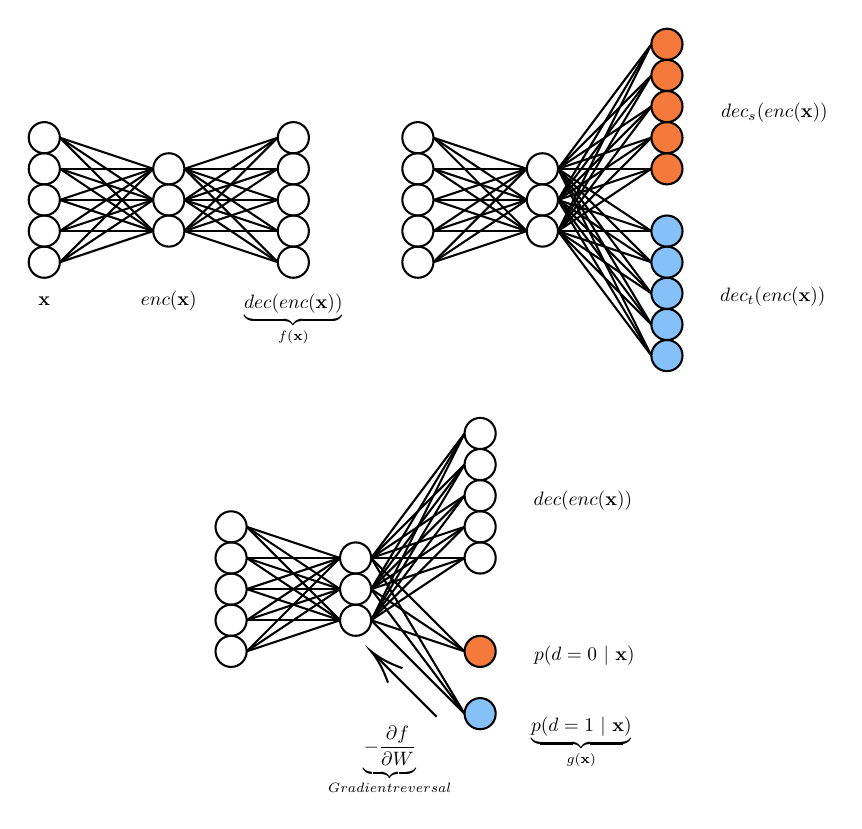
\begin{tikzpicture}[x=0.75pt,y=0.75pt,yscale=-1.5,xscale=1.5]
%uncomment if require: \path (0,276); %set diagram left start at 0, and has height of 276

%Straight Lines [id:da24666910276810683] 
\draw    (140,40) -- (170,50) ;


%Straight Lines [id:da697879806591556] 
\draw    (140,40) -- (170,70) ;


%Straight Lines [id:da45653170744759564] 
\draw    (140,50) -- (170,50) ;


%Straight Lines [id:da24640626203600113] 
\draw    (140,50) -- (170,70) ;


%Straight Lines [id:da14428496650149336] 
\draw    (140,40) -- (170,60) ;


%Straight Lines [id:da49974731754300594] 
\draw    (140,50) -- (170,60) ;


%Straight Lines [id:da9614556788875354] 
\draw    (140,60) -- (170,50) ;


%Straight Lines [id:da10534458725346374] 
\draw    (140,60) -- (170,60) ;


%Straight Lines [id:da543461087491177] 
\draw    (140,60) -- (170,70) ;


%Straight Lines [id:da4292705270352881] 
\draw    (140,70) -- (170,50) ;


%Straight Lines [id:da03639305677867266] 
\draw    (140,70) -- (170,60) ;


%Straight Lines [id:da22840220022169055] 
\draw    (140,70) -- (170,70) ;


%Straight Lines [id:da4033338734327042] 
\draw    (140,80) -- (170,50) ;


%Straight Lines [id:da44817655533184564] 
\draw    (140,80) -- (170,60) ;


%Straight Lines [id:da8978932818688041] 
\draw    (140,80) -- (170,70) ;


%Straight Lines [id:da6539941786163147] 
\draw    (180,50) -- (210,10) ;


%Straight Lines [id:da4228461714581967] 
\draw    (180,50) -- (210,20) ;


%Straight Lines [id:da9026703943765524] 
\draw    (180,50) -- (210,30) ;


%Straight Lines [id:da6189630704708299] 
\draw    (180,50) -- (210,40) ;


%Straight Lines [id:da5857421217089592] 
\draw    (180,50) -- (210,50) ;


%Straight Lines [id:da9731776866766855] 
\draw    (180,60) -- (210,10) ;


%Straight Lines [id:da26125864793761233] 
\draw    (180,60) -- (210,20) ;


%Straight Lines [id:da6299294938770524] 
\draw    (180,60) -- (210,30) ;


%Straight Lines [id:da08604593003679761] 
\draw    (180,60) -- (210,40) ;


%Straight Lines [id:da3551821383636762] 
\draw    (180,60) -- (210,50) ;


%Straight Lines [id:da01644536702904964] 
\draw    (180,70) -- (210,10) ;


%Straight Lines [id:da08984782168002814] 
\draw    (180,70) -- (210,20) ;


%Straight Lines [id:da7297854507434446] 
\draw    (180,70) -- (210,30) ;


%Straight Lines [id:da28712519568669226] 
\draw    (180,70) -- (210,40) ;


%Straight Lines [id:da7339411459924542] 
\draw    (180,70) -- (210,50) ;


%Straight Lines [id:da032201283792261726] 
\draw    (180,70) -- (210,70) ;


%Straight Lines [id:da7424076051937555] 
\draw    (180,70) -- (210,80) ;


%Straight Lines [id:da41463826623920286] 
\draw    (180,70) -- (210,90) ;


%Straight Lines [id:da2809630474861802] 
\draw    (180,70) -- (210,100) ;


%Straight Lines [id:da7475122527824513] 
\draw    (180,70) -- (210,110) ;


%Straight Lines [id:da7391877419728995] 
\draw    (180,50) -- (210,70) ;


%Straight Lines [id:da8977794676806864] 
\draw    (180,50) -- (210,80) ;


%Straight Lines [id:da0010718049207566471] 
\draw    (180,50) -- (210,90) ;


%Straight Lines [id:da8626930927677362] 
\draw    (180,50) -- (210,100) ;


%Straight Lines [id:da9954138759190354] 
\draw    (180,50) -- (210,110) ;


%Straight Lines [id:da16443791998465473] 
\draw    (180,60) -- (210,70) ;


%Straight Lines [id:da9045174439769256] 
\draw    (180,60) -- (210,80) ;


%Straight Lines [id:da22632577339975046] 
\draw    (180,60) -- (210,90) ;


%Straight Lines [id:da5026137310053356] 
\draw    (180,60) -- (210,100) ;


%Straight Lines [id:da42010050551965605] 
\draw    (180,60) -- (210,110) ;


%Shape: Circle [id:dp9610723962373001] 
\draw   (130,40) .. controls (130,37.24) and (132.24,35) .. (135,35) .. controls (137.76,35) and (140,37.24) .. (140,40) .. controls (140,42.76) and (137.76,45) .. (135,45) .. controls (132.24,45) and (130,42.76) .. (130,40) -- cycle ;
%Shape: Circle [id:dp4241528934798183] 
\draw   (140,80) .. controls (140,77.24) and (137.76,75) .. (135,75) .. controls (132.24,75) and (130,77.24) .. (130,80) .. controls (130,82.76) and (132.24,85) .. (135,85) .. controls (137.76,85) and (140,82.76) .. (140,80) -- cycle ;
%Shape: Circle [id:dp8823014196681026] 
\draw   (140,70) .. controls (140,67.24) and (137.76,65) .. (135,65) .. controls (132.24,65) and (130,67.24) .. (130,70) .. controls (130,72.76) and (132.24,75) .. (135,75) .. controls (137.76,75) and (140,72.76) .. (140,70) -- cycle ;
%Shape: Circle [id:dp8588767105930342] 
\draw   (140,50) .. controls (140,47.24) and (137.76,45) .. (135,45) .. controls (132.24,45) and (130,47.24) .. (130,50) .. controls (130,52.76) and (132.24,55) .. (135,55) .. controls (137.76,55) and (140,52.76) .. (140,50) -- cycle ;
%Shape: Circle [id:dp7099955212296606] 
\draw   (140,60) .. controls (140,57.24) and (137.76,55) .. (135,55) .. controls (132.24,55) and (130,57.24) .. (130,60) .. controls (130,62.76) and (132.24,65) .. (135,65) .. controls (137.76,65) and (140,62.76) .. (140,60) -- cycle ;
%Shape: Circle [id:dp35196457014447435] 
\draw  [fill={rgb, 255:red, 133; green, 192; blue, 249 }  ,fill opacity=1 ] (210,70) .. controls (210,67.24) and (212.24,65) .. (215,65) .. controls (217.76,65) and (220,67.24) .. (220,70) .. controls (220,72.76) and (217.76,75) .. (215,75) .. controls (212.24,75) and (210,72.76) .. (210,70) -- cycle ;
%Shape: Circle [id:dp3350351238334317] 
\draw  [fill={rgb, 255:red, 133; green, 192; blue, 249 }  ,fill opacity=1 ] (220,110) .. controls (220,107.24) and (217.76,105) .. (215,105) .. controls (212.24,105) and (210,107.24) .. (210,110) .. controls (210,112.76) and (212.24,115) .. (215,115) .. controls (217.76,115) and (220,112.76) .. (220,110) -- cycle ;
%Shape: Circle [id:dp9135073008422223] 
\draw  [fill={rgb, 255:red, 133; green, 192; blue, 249 }  ,fill opacity=1 ] (220,100) .. controls (220,97.24) and (217.76,95) .. (215,95) .. controls (212.24,95) and (210,97.24) .. (210,100) .. controls (210,102.76) and (212.24,105) .. (215,105) .. controls (217.76,105) and (220,102.76) .. (220,100) -- cycle ;
%Shape: Circle [id:dp8905172808557287] 
\draw  [fill={rgb, 255:red, 133; green, 192; blue, 249 }  ,fill opacity=1 ] (220,80) .. controls (220,77.24) and (217.76,75) .. (215,75) .. controls (212.24,75) and (210,77.24) .. (210,80) .. controls (210,82.76) and (212.24,85) .. (215,85) .. controls (217.76,85) and (220,82.76) .. (220,80) -- cycle ;
%Shape: Circle [id:dp6181164826875234] 
\draw  [fill={rgb, 255:red, 133; green, 192; blue, 249 }  ,fill opacity=1 ] (220,90) .. controls (220,87.24) and (217.76,85) .. (215,85) .. controls (212.24,85) and (210,87.24) .. (210,90) .. controls (210,92.76) and (212.24,95) .. (215,95) .. controls (217.76,95) and (220,92.76) .. (220,90) -- cycle ;
%Shape: Circle [id:dp1520895910431196] 
\draw  [fill={rgb, 255:red, 245; green, 121; blue, 58 }  ,fill opacity=1 ] (210,10) .. controls (210,7.24) and (212.24,5) .. (215,5) .. controls (217.76,5) and (220,7.24) .. (220,10) .. controls (220,12.76) and (217.76,15) .. (215,15) .. controls (212.24,15) and (210,12.76) .. (210,10) -- cycle ;
%Shape: Circle [id:dp7026702488374332] 
\draw  [fill={rgb, 255:red, 245; green, 121; blue, 58 }  ,fill opacity=1 ] (220,50) .. controls (220,47.24) and (217.76,45) .. (215,45) .. controls (212.24,45) and (210,47.24) .. (210,50) .. controls (210,52.76) and (212.24,55) .. (215,55) .. controls (217.76,55) and (220,52.76) .. (220,50) -- cycle ;
%Shape: Circle [id:dp5213329246754517] 
\draw  [fill={rgb, 255:red, 245; green, 121; blue, 58 }  ,fill opacity=1 ] (220,40) .. controls (220,37.24) and (217.76,35) .. (215,35) .. controls (212.24,35) and (210,37.24) .. (210,40) .. controls (210,42.76) and (212.24,45) .. (215,45) .. controls (217.76,45) and (220,42.76) .. (220,40) -- cycle ;
%Shape: Circle [id:dp5786956728255837] 
\draw  [fill={rgb, 255:red, 245; green, 121; blue, 58 }  ,fill opacity=1 ] (220,20) .. controls (220,17.24) and (217.76,15) .. (215,15) .. controls (212.24,15) and (210,17.24) .. (210,20) .. controls (210,22.76) and (212.24,25) .. (215,25) .. controls (217.76,25) and (220,22.76) .. (220,20) -- cycle ;
%Shape: Circle [id:dp5821617344416693] 
\draw  [fill={rgb, 255:red, 245; green, 121; blue, 58 }  ,fill opacity=1 ] (220,30) .. controls (220,27.24) and (217.76,25) .. (215,25) .. controls (212.24,25) and (210,27.24) .. (210,30) .. controls (210,32.76) and (212.24,35) .. (215,35) .. controls (217.76,35) and (220,32.76) .. (220,30) -- cycle ;
%Shape: Circle [id:dp4172765671827007] 
\draw   (170,50) .. controls (170,47.24) and (172.24,45) .. (175,45) .. controls (177.76,45) and (180,47.24) .. (180,50) .. controls (180,52.76) and (177.76,55) .. (175,55) .. controls (172.24,55) and (170,52.76) .. (170,50) -- cycle ;
%Shape: Circle [id:dp07503304030856917] 
\draw   (180,60) .. controls (180,57.24) and (177.76,55) .. (175,55) .. controls (172.24,55) and (170,57.24) .. (170,60) .. controls (170,62.76) and (172.24,65) .. (175,65) .. controls (177.76,65) and (180,62.76) .. (180,60) -- cycle ;
%Shape: Circle [id:dp2088383902581149] 
\draw   (180,70) .. controls (180,67.24) and (177.76,65) .. (175,65) .. controls (172.24,65) and (170,67.24) .. (170,70) .. controls (170,72.76) and (172.24,75) .. (175,75) .. controls (177.76,75) and (180,72.76) .. (180,70) -- cycle ;
%Straight Lines [id:da44477109133134207] 
\draw    (20,40) -- (50,50) ;


%Straight Lines [id:da06851739836367998] 
\draw    (20,40) -- (50,70) ;


%Straight Lines [id:da04676410664055464] 
\draw    (20,50) -- (50,50) ;


%Straight Lines [id:da32865342870114234] 
\draw    (20,50) -- (50,70) ;


%Straight Lines [id:da0320256266686898] 
\draw    (20,40) -- (50,60) ;


%Straight Lines [id:da9745372402149663] 
\draw    (20,50) -- (50,60) ;


%Straight Lines [id:da5113930130914643] 
\draw    (20,60) -- (50,50) ;


%Straight Lines [id:da5491533551363393] 
\draw    (20,60) -- (50,60) ;


%Straight Lines [id:da364225402818816] 
\draw    (20,60) -- (50,70) ;


%Straight Lines [id:da10360301870329192] 
\draw    (20,70) -- (50,50) ;


%Straight Lines [id:da8647679120583445] 
\draw    (20,70) -- (50,60) ;


%Straight Lines [id:da8744645806377251] 
\draw    (20,70) -- (50,70) ;


%Straight Lines [id:da007028015998127302] 
\draw    (20,80) -- (50,50) ;


%Straight Lines [id:da5490722094989353] 
\draw    (20,80) -- (50,60) ;


%Straight Lines [id:da19708378694605655] 
\draw    (20,80) -- (50,70) ;


%Straight Lines [id:da7256753801437874] 
\draw    (60,50) -- (90,40) ;


%Straight Lines [id:da5072756751895783] 
\draw    (60,50) -- (90,50) ;


%Straight Lines [id:da23683919330537717] 
\draw    (60,50) -- (90,60) ;


%Straight Lines [id:da26745674265851405] 
\draw    (60,50) -- (90,70) ;


%Straight Lines [id:da9365583724273878] 
\draw    (60,50) -- (90,80) ;


%Straight Lines [id:da18841020914078122] 
\draw    (60,60) -- (90,40) ;


%Straight Lines [id:da8947710179904554] 
\draw    (60,60) -- (90,50) ;


%Straight Lines [id:da7503785372644488] 
\draw    (60,60) -- (90,70) ;


%Straight Lines [id:da6045213186209335] 
\draw    (60,60) -- (90,80) ;


%Straight Lines [id:da0027664899274344457] 
\draw    (60,70) -- (90,40) ;


%Straight Lines [id:da19382466738982462] 
\draw    (60,70) -- (90,50) ;


%Straight Lines [id:da711342164443469] 
\draw    (60,70) -- (90,60) ;


%Straight Lines [id:da16207278960263516] 
\draw    (60,70) -- (90,70) ;


%Straight Lines [id:da8413138977113539] 
\draw    (60,70) -- (90,80) ;


%Shape: Circle [id:dp4048067870630523] 
\draw   (10,40) .. controls (10,37.24) and (12.24,35) .. (15,35) .. controls (17.76,35) and (20,37.24) .. (20,40) .. controls (20,42.76) and (17.76,45) .. (15,45) .. controls (12.24,45) and (10,42.76) .. (10,40) -- cycle ;
%Shape: Circle [id:dp2851403134074575] 
\draw   (20,80) .. controls (20,77.24) and (17.76,75) .. (15,75) .. controls (12.24,75) and (10,77.24) .. (10,80) .. controls (10,82.76) and (12.24,85) .. (15,85) .. controls (17.76,85) and (20,82.76) .. (20,80) -- cycle ;
%Shape: Circle [id:dp4433685057389867] 
\draw   (20,70) .. controls (20,67.24) and (17.76,65) .. (15,65) .. controls (12.24,65) and (10,67.24) .. (10,70) .. controls (10,72.76) and (12.24,75) .. (15,75) .. controls (17.76,75) and (20,72.76) .. (20,70) -- cycle ;
%Shape: Circle [id:dp4106041397721897] 
\draw   (20,50) .. controls (20,47.24) and (17.76,45) .. (15,45) .. controls (12.24,45) and (10,47.24) .. (10,50) .. controls (10,52.76) and (12.24,55) .. (15,55) .. controls (17.76,55) and (20,52.76) .. (20,50) -- cycle ;
%Shape: Circle [id:dp3785752657258068] 
\draw   (20,60) .. controls (20,57.24) and (17.76,55) .. (15,55) .. controls (12.24,55) and (10,57.24) .. (10,60) .. controls (10,62.76) and (12.24,65) .. (15,65) .. controls (17.76,65) and (20,62.76) .. (20,60) -- cycle ;
%Shape: Circle [id:dp3545561612181919] 
\draw   (50,50) .. controls (50,47.24) and (52.24,45) .. (55,45) .. controls (57.76,45) and (60,47.24) .. (60,50) .. controls (60,52.76) and (57.76,55) .. (55,55) .. controls (52.24,55) and (50,52.76) .. (50,50) -- cycle ;
%Shape: Circle [id:dp03184569393344261] 
\draw   (60,60) .. controls (60,57.24) and (57.76,55) .. (55,55) .. controls (52.24,55) and (50,57.24) .. (50,60) .. controls (50,62.76) and (52.24,65) .. (55,65) .. controls (57.76,65) and (60,62.76) .. (60,60) -- cycle ;
%Shape: Circle [id:dp09767100194788203] 
\draw   (60,70) .. controls (60,67.24) and (57.76,65) .. (55,65) .. controls (52.24,65) and (50,67.24) .. (50,70) .. controls (50,72.76) and (52.24,75) .. (55,75) .. controls (57.76,75) and (60,72.76) .. (60,70) -- cycle ;
%Shape: Circle [id:dp9329614439307907] 
\draw   (90,40) .. controls (90,37.24) and (92.24,35) .. (95,35) .. controls (97.76,35) and (100,37.24) .. (100,40) .. controls (100,42.76) and (97.76,45) .. (95,45) .. controls (92.24,45) and (90,42.76) .. (90,40) -- cycle ;
%Shape: Circle [id:dp3738220778976774] 
\draw   (100,80) .. controls (100,77.24) and (97.76,75) .. (95,75) .. controls (92.24,75) and (90,77.24) .. (90,80) .. controls (90,82.76) and (92.24,85) .. (95,85) .. controls (97.76,85) and (100,82.76) .. (100,80) -- cycle ;
%Shape: Circle [id:dp37601692135403886] 
\draw   (100,70) .. controls (100,67.24) and (97.76,65) .. (95,65) .. controls (92.24,65) and (90,67.24) .. (90,70) .. controls (90,72.76) and (92.24,75) .. (95,75) .. controls (97.76,75) and (100,72.76) .. (100,70) -- cycle ;
%Shape: Circle [id:dp8849044250507954] 
\draw   (100,50) .. controls (100,47.24) and (97.76,45) .. (95,45) .. controls (92.24,45) and (90,47.24) .. (90,50) .. controls (90,52.76) and (92.24,55) .. (95,55) .. controls (97.76,55) and (100,52.76) .. (100,50) -- cycle ;
%Shape: Circle [id:dp9368423036800632] 
\draw   (100,60) .. controls (100,57.24) and (97.76,55) .. (95,55) .. controls (92.24,55) and (90,57.24) .. (90,60) .. controls (90,62.76) and (92.24,65) .. (95,65) .. controls (97.76,65) and (100,62.76) .. (100,60) -- cycle ;
%Straight Lines [id:da6800286081737521] 
\draw    (60,60) -- (90,60) ;


%Straight Lines [id:da6159247490010764] 
\draw    (80,165) -- (110,175) ;


%Straight Lines [id:da023906701840495148] 
\draw    (80,165) -- (110,195) ;


%Straight Lines [id:da9532403392384969] 
\draw    (80,175) -- (110,175) ;


%Straight Lines [id:da0003735557756083807] 
\draw    (80,175) -- (110,195) ;


%Straight Lines [id:da5010402304603807] 
\draw    (80,165) -- (110,185) ;


%Straight Lines [id:da8725238972861316] 
\draw    (80,175) -- (110,185) ;


%Straight Lines [id:da5375250396189268] 
\draw    (80,185) -- (110,175) ;


%Straight Lines [id:da725924491175131] 
\draw    (80,185) -- (110,185) ;


%Straight Lines [id:da04111371617980086] 
\draw    (80,185) -- (110,195) ;


%Straight Lines [id:da33499213229153124] 
\draw    (80,195) -- (110,175) ;


%Straight Lines [id:da45016356585290995] 
\draw    (80,195) -- (110,185) ;


%Straight Lines [id:da8047431702676948] 
\draw    (80,195) -- (110,195) ;


%Straight Lines [id:da28826002249006477] 
\draw    (80,205) -- (110,175) ;


%Straight Lines [id:da5206435322631933] 
\draw    (80,205) -- (110,185) ;


%Straight Lines [id:da9017552252066877] 
\draw    (80,205) -- (110,195) ;


%Straight Lines [id:da8675855391162514] 
\draw    (120,175) -- (150,135) ;


%Straight Lines [id:da6204357086098623] 
\draw    (120,175) -- (150,145) ;


%Straight Lines [id:da752453318054359] 
\draw    (120,175) -- (150,155) ;


%Straight Lines [id:da6680600683275931] 
\draw    (120,175) -- (150,165) ;


%Straight Lines [id:da5869969506314183] 
\draw    (120,175) -- (150,175) ;


%Straight Lines [id:da8254777914375734] 
\draw    (120,185) -- (150,135) ;


%Straight Lines [id:da9276862779850157] 
\draw    (120,185) -- (150,145) ;


%Straight Lines [id:da4581484513109556] 
\draw    (120,185) -- (150,155) ;


%Straight Lines [id:da8096514994492826] 
\draw    (120,185) -- (150,165) ;


%Straight Lines [id:da6056653554111322] 
\draw    (120,185) -- (150,175) ;


%Straight Lines [id:da7218427728660654] 
\draw    (120,195) -- (150,135) ;


%Straight Lines [id:da36287396394413307] 
\draw    (120,195) -- (150,145) ;


%Straight Lines [id:da826903652012305] 
\draw    (120,195) -- (150,155) ;


%Straight Lines [id:da9038375906077686] 
\draw    (120,195) -- (150,165) ;


%Straight Lines [id:da7449615359848694] 
\draw    (120,195) -- (150,175) ;


%Straight Lines [id:da09954171266085299] 
\draw    (120,175) -- (150,205) ;


%Straight Lines [id:da08890024604491509] 
\draw    (120,175) -- (150,225) ;


%Straight Lines [id:da8941620194091715] 
\draw    (120,185) -- (150,205) ;


%Straight Lines [id:da9882879025797193] 
\draw    (120,195) -- (150,205) ;


%Straight Lines [id:da5118070293168346] 
\draw    (120,185) -- (150,225) ;


%Straight Lines [id:da7063672649828733] 
\draw    (120,195) -- (150,225) ;


%Straight Lines [id:da2774771727684625] 
\draw [color={rgb, 255:red, 0; green, 0; blue, 0 }  ,draw opacity=1 ]   (141,226) -- (121.41,206.41) ;
\draw [shift={(120,205)}, rotate = 405] [color={rgb, 255:red, 0; green, 0; blue, 0 }  ,draw opacity=1 ][line width=0.75]    (10.93,-3.29) .. controls (6.95,-1.4) and (3.31,-0.3) .. (0,0) .. controls (3.31,0.3) and (6.95,1.4) .. (10.93,3.29)   ;

%Shape: Circle [id:dp03877052736761255] 
\draw   (70,165) .. controls (70,162.24) and (72.24,160) .. (75,160) .. controls (77.76,160) and (80,162.24) .. (80,165) .. controls (80,167.76) and (77.76,170) .. (75,170) .. controls (72.24,170) and (70,167.76) .. (70,165) -- cycle ;
%Shape: Circle [id:dp5808274445829077] 
\draw   (80,205) .. controls (80,202.24) and (77.76,200) .. (75,200) .. controls (72.24,200) and (70,202.24) .. (70,205) .. controls (70,207.76) and (72.24,210) .. (75,210) .. controls (77.76,210) and (80,207.76) .. (80,205) -- cycle ;
%Shape: Circle [id:dp8162710162508374] 
\draw   (80,195) .. controls (80,192.24) and (77.76,190) .. (75,190) .. controls (72.24,190) and (70,192.24) .. (70,195) .. controls (70,197.76) and (72.24,200) .. (75,200) .. controls (77.76,200) and (80,197.76) .. (80,195) -- cycle ;
%Shape: Circle [id:dp9941665107203423] 
\draw   (80,175) .. controls (80,172.24) and (77.76,170) .. (75,170) .. controls (72.24,170) and (70,172.24) .. (70,175) .. controls (70,177.76) and (72.24,180) .. (75,180) .. controls (77.76,180) and (80,177.76) .. (80,175) -- cycle ;
%Shape: Circle [id:dp633788624475869] 
\draw   (80,185) .. controls (80,182.24) and (77.76,180) .. (75,180) .. controls (72.24,180) and (70,182.24) .. (70,185) .. controls (70,187.76) and (72.24,190) .. (75,190) .. controls (77.76,190) and (80,187.76) .. (80,185) -- cycle ;
%Shape: Circle [id:dp7410501614236662] 
\draw   (150,135) .. controls (150,132.24) and (152.24,130) .. (155,130) .. controls (157.76,130) and (160,132.24) .. (160,135) .. controls (160,137.76) and (157.76,140) .. (155,140) .. controls (152.24,140) and (150,137.76) .. (150,135) -- cycle ;
%Shape: Circle [id:dp308486328424064] 
\draw   (160,175) .. controls (160,172.24) and (157.76,170) .. (155,170) .. controls (152.24,170) and (150,172.24) .. (150,175) .. controls (150,177.76) and (152.24,180) .. (155,180) .. controls (157.76,180) and (160,177.76) .. (160,175) -- cycle ;
%Shape: Circle [id:dp8868128856352178] 
\draw   (160,165) .. controls (160,162.24) and (157.76,160) .. (155,160) .. controls (152.24,160) and (150,162.24) .. (150,165) .. controls (150,167.76) and (152.24,170) .. (155,170) .. controls (157.76,170) and (160,167.76) .. (160,165) -- cycle ;
%Shape: Circle [id:dp4050611092738252] 
\draw   (160,145) .. controls (160,142.24) and (157.76,140) .. (155,140) .. controls (152.24,140) and (150,142.24) .. (150,145) .. controls (150,147.76) and (152.24,150) .. (155,150) .. controls (157.76,150) and (160,147.76) .. (160,145) -- cycle ;
%Shape: Circle [id:dp2141694033042939] 
\draw   (160,155) .. controls (160,152.24) and (157.76,150) .. (155,150) .. controls (152.24,150) and (150,152.24) .. (150,155) .. controls (150,157.76) and (152.24,160) .. (155,160) .. controls (157.76,160) and (160,157.76) .. (160,155) -- cycle ;
%Shape: Circle [id:dp9491693550654471] 
\draw   (110,175) .. controls (110,172.24) and (112.24,170) .. (115,170) .. controls (117.76,170) and (120,172.24) .. (120,175) .. controls (120,177.76) and (117.76,180) .. (115,180) .. controls (112.24,180) and (110,177.76) .. (110,175) -- cycle ;
%Shape: Circle [id:dp6566208271952009] 
\draw   (120,185) .. controls (120,182.24) and (117.76,180) .. (115,180) .. controls (112.24,180) and (110,182.24) .. (110,185) .. controls (110,187.76) and (112.24,190) .. (115,190) .. controls (117.76,190) and (120,187.76) .. (120,185) -- cycle ;
%Shape: Circle [id:dp7358420255402347] 
\draw   (120,195) .. controls (120,192.24) and (117.76,190) .. (115,190) .. controls (112.24,190) and (110,192.24) .. (110,195) .. controls (110,197.76) and (112.24,200) .. (115,200) .. controls (117.76,200) and (120,197.76) .. (120,195) -- cycle ;
%Shape: Circle [id:dp8741754452542158] 
\draw  [fill={rgb, 255:red, 133; green, 192; blue, 249 }  ,fill opacity=1 ] (160,225) .. controls (160,222.24) and (157.76,220) .. (155,220) .. controls (152.24,220) and (150,222.24) .. (150,225) .. controls (150,227.76) and (152.24,230) .. (155,230) .. controls (157.76,230) and (160,227.76) .. (160,225) -- cycle ;
%Shape: Circle [id:dp08442203504236712] 
\draw  [fill={rgb, 255:red, 245; green, 121; blue, 58 }  ,fill opacity=1 ] (160,205) .. controls (160,202.24) and (157.76,200) .. (155,200) .. controls (152.24,200) and (150,202.24) .. (150,205) .. controls (150,207.76) and (152.24,210) .. (155,210) .. controls (157.76,210) and (160,207.76) .. (160,205) -- cycle ;

% Text Node
\draw (15,92.5) node [scale=0.7]  {$\mathbf{x}$};
% Text Node
\draw (55,92.5) node [scale=0.7]  {$enc(\mathbf{x})$};
% Text Node
\draw (95,98.5) node [scale=0.7]  {$\underbrace{dec( enc(\mathbf{x}))}_{f(\mathbf{x})}$};
% Text Node
\draw (249.5,32) node [scale=0.7]  {$dec_{s}( enc(\mathbf{x}))$};
% Text Node
\draw (249,91) node [scale=0.7]  {$dec_{t}( enc(\mathbf{x}))$};
% Text Node
\draw (126,240) node [scale=0.7]  {$\underbrace{-\frac{\partial f}{\partial W}}_{\text{Gradient reversal}}$};
% Text Node
\draw (188,156.5) node [scale=0.7]  {$dec( enc(\mathbf{x}))$};
% Text Node
\draw (188.5,206.5) node [scale=0.7]  {$p( d=0\ |\ \mathbf{x})$};
% Text Node
\draw (187.5,234.5) node [scale=0.7]  {$\underbrace{p( d=1\ |\ \mathbf{x})}_{g(\mathbf{x})}$};
\end{tikzpicture}
\caption{Multitask autoencoders used for dimensionality reduction over multi-cell-line data. Clockwise from top left: vanilla autoencoder, multitask autoencoder, and domain-adversarial autoencoder. Colouring indicates separate treatment of each domain (cell line).}
\label{fig:architectures}
\end{figure}

\subsection{Model evaluation}

We compared different profiling settings by evaluating performance on a MOA prediction task. For this, we balanced our datasets by randomly sampling five drugs from each of the 8 classes specified in Section \ref{sec:data}, analysing 40 drugs at a time. Applying the LOCOCV scheme described in Section \ref{subsec:moa_prediction}, we note that random accuracy is $12.5\%$. To account for random variability, we repeated LOCOCV 60 times with different sets of randomly sampled drugs and in Section \ref{sec:results} report average top-1 accuracy and standard deviation as the percentage of MOAs correctly predicted by the 1-NN classifier. We consider this to be a more rigorous approach in a comparative study, as while a given method often fit one drug set well, it was harder to find hyperparameter choices that worked well across all sets. We used a Wilcoxon signed-rank test to establish significance against baselines over the 60 rounds.

\subsection{Software}

We use Cell Cognition \cite{held2010cellcognition} to perform the first stages of the classical analysis pipeline, namely, image preprocessing, cell segmentation and feature extraction.

All models were coded using the \texttt{scikit-learn} \cite{scikit-learn} and \texttt{Keras} \cite{chollet2015keras} frameworks for Python, unless otherwise noted\footnote{Worked examples of code and feature data available at \texttt{https://github.com/jcboyd/multi-cell-line}}. Basic image processing was performed with \texttt{scikit-image} \cite{VanderWalt2014}. 

\section{Results}
\label{sec:results}

In Section \ref{subsec:single} we evaluate a range of approaches to dimensionality reduction--as described in Section \ref{subsubsec:dimensionality_reduction}--on their utility in creating cell representations that aggregate into discriminative phenotypic profiles for MOA prediction. This we do in separate single-cell-line experiments. In Section \ref{subsubsec:predictionmulticellline} we show how our best performing model on single-cell-line data--the autoencoder--may be extended for multi-cell-line analysis, providing comparisons for learning on handcrafted features, as well as raw pixels. We then illustrate how our optimised phenotypic profile design can be used to identify differential drug effects between cell lines across our entire drug panel in Section \ref{subsubsec:differential}. In Section \ref{subsubsec:accumulating} we explore how the effect of adding cell lines to an analysis effects MOA predictability.

%The results are summarized in table \ref{table:joint}. 

% \begin{table*}[!t]
% \processtable{Comparison of performance for models arranged by profile criterion category. \label{Tab:01}} {\begin{tabular}{@{}lllll@{}}\toprule Property & Approach & MDA231 accuracy ($\mu, \sigma$) & MDA468 accuracy ($\mu, \sigma$) & Joint accuracy ($\mu, \sigma$) \\\midrule
% Unit of measurement & Cell bounding box & 29.67, 6.35 & 23.63, 6.49 & 34.42, 7.02 \\
%  & Grid ($4\times6$) & 31.04, 7.12 & 18.86, 5.71 & 30.5, 5.64 \\
%  & Grid ($10\times12$) & \color{red}{31.20, 6.41} & \color{red}{27.08, 6.13} & 34.42, 6.35 \\
%  & Full image & 25.33, 6.49 & 16.08, 3.91 & 34.63, 6.66 \\\midrule
% Feature representation & Handcrafted & 18.58, 5.66 & 20.08, 4.53 & 21.63, 5.66 \\
%  & ResNet50 & 29.67, 6.35 & 23.63, 6.49 & 34.42, 7.02 \\\midrule
% Dimensionality reduction & PCA + whitening & 18.58, 5.62 & 20.08, 4.49 & - \\
%  & Hierarchical clustering & 11.77, 5.65 & 16.71, 6.63 & - \\
%  & K-means & 15.42, 6.73 & 16.71, 6.79 & - \\
%  & GMM & 15.73, 6.63 & 17.23, 6.24 & - \\
%  & Convolutional autoencoder & 19.13, 6.96 & 14.21, 5.41 & - \\
%  & Multiple-instance learning & 19.51, 9.95 & 16.81, 8.16 & - \\
%  & MCNN & 12.29, 11.15 & 12.08, 12.71 & \\
%  & Autoencoder & 10.56, 5.07 & 15.58, 6.67 & 28.13, 7.30 \\
%  & Multi-input autoencoder & - & - & 31.21, 6.63 \\
%  & Multitask autoencoder & - & - & 32.04, 6.88 \\
%  & Domain-adversarial autoencoder & & & \color{red}{35.67, 6.94} \\\midrule
% Aggregation strategy & K-S test & 19.08, 5.09 & 20.17, 6.21 & - \\
%  & Averaging & 18.58, 5.66 & 20.08, 4.53 & 21.63, 5.66 \\
%  & Norm to hyperplane & 17.38, 4.99 & 17.40, 5.26 & - \\\botrule
% \end{tabular}}{}
% \label{table:joint}
% \end{table*}



%In comparison with other datasets, \cite{adams2006compound} used 51 drugs in 13 MOA categories, \cite{slack2008characterizing} used 35 drugs in six MOA categories, and the widely studied BBBC dataset consists of 39 drugs in 13 categories. The main difference is that our own MOA classes are less heterogeneous, mounting a greater bioinformatic challenge than the standard benchmark datasets Broad Institute Benchmark Collection 21 (BBBC21v2) (\cite{ljosa2012annotated}) used in \cite{kandaswamy2016high} and \cite{godinez2017multi}, where even a simple model can be extremely effective. For example, \cite{singh2014pipeline} achieved $90\%$ accuracy with element-wise averaging of hand-crafted features after a simple luminosity correction.

\subsection{Single cell line analysis}
\label{subsec:single}

%\begin{figure}
%  \includegraphics[width=\linewidth]{img/clustermap.pdf}
%  \caption{Clustermap of Ward clustering and adjusted Rand score of ??}
%\end{figure}

%\subsubsection{Measurement unit and feature representation}
%\label{ref:unit_results}
%
%In Table \ref{table:unit}, we compare profiles developed under different measurement units along with different feature representations: segmented nuclei represented by handcrafted features (HC), ResNet50 features (RN50), and features learned directly from raw pixels by a convolutional autoencoder (CAE); image patches from coarse $4 \times 6$ and fine $10 \times 12$ grids represented by ResNet50 features; and finally entire images, represented by ResNet50 and MCNN.
%
%\begin{table}[!ht]
%\processtable{Comparison of performance of approaches with and without segmentation and corresponding representations. We show mean and standard deviations of accuracies over 60 runs.
%%\label{Tab:01}
%}
%{
%\begin{tabular}{@{}lll@{}}
%\toprule Approach & MDA231 accuracy ($\mu$, $\sigma$)  & MDA468 accuracy ($\mu$, $\sigma$)\\\midrule
%Segmentation (HC) & $18.58, 5.62$ & $20.08, 4.49$ \\
%Segmentation (CAE) & $19.13, 6.96$ & $14.21, 5.41$\\
%Segmentation (RN50) & $29.67, 6.35$ & $23.63, 6.49$ \\
%Grid $10\times12$ (RN50) & $\mathbf{31.20, 6.41}$ & $\mathbf{27.08, 6.13}$\\
%Grid $4\times6$ (RN50) & $31.04, 7.12$ & $18.86, 5.71$ \\
%Full image (RN50) & $25.33, 6.49$ & $16.08, 3.91$ \\
%Full image (MCNN) & $16.92, 5.54$ & $14.33, 4.81$ \\\botrule
%\label{table:unit}
%\end{tabular}}{}
%\end{table}
%
%We first observe that pre-trained ResNet50 features outperform handcrafted features across virtually all measurement units. Learned representations (CAE and MCNN) find some signal and exceed random performance, but on average perform less well than either. Secondly, we see that segmentation does not bring an advantage with respect to patch-based approaches. However, we do observe that image patches in a fine grid yield the best overall result. Notably, 120 patches was chosen to approximate the average number of cells per image field. We therefore conclude that while segmentation may not be crucial, the cellular scale is--depending on the cell line--presumably the relevant one.
% 
%We speculate that the improvement of a grid-based approach over cell segmentation for RN50 features may be due to capturing drug viability. The viability $v = \frac{n^d}{n^-}$ of a drug refers to the change in the population size $n^d$ relative to that of the negative control $n^-$. When cells are segmented, the viability of a drug is implied by the cell sample size, though this information may be lost in the downstream aggregation step. When cells are not explicitly segmented, the viability is represented indirectly by how populated the field is. Viability may be an important phenotypic characteristic of a drug effect.
%
%%For the majority of approaches this is the segmented cell. Cell nuclei are segmented on the DAPI channel by subtracting a background image formed with a mean filter, before clipping to zero. Touching nuclei are then further separated by applying the watershed transform on the inverse distance map of the foreground image. The cytoplasm is segmented from the microtubule channel (Cy5) following \cite{jones2005voronoi}. This yields an average of $\sim10^5$ cells for each cell line. It is from the segmented cells alone that we extract handcrafted features (see \ref{subsubsec:feat_results})).
%
%%We also extract pre-trained features from segmented cells. To do this, we take image crops of cells formed by padding the bounding boxes of the segmented nuclei to a common size ($128\times 128$px) and performing bilinear downsampling to produce $32 \times 32 \times 3$ inputs. \twcomment{Unclear why we do this.} We also use these as the inputs to the convolutional autoencoder. We use the final convolutional layer of ResNet50 pre-trained on ImageNet data as a feature extractor on the same crops, and also patches of fixed size. This produces a CNN code feature vector of $2048$ elements for each cell. In addition, we study the performance of segmentation-free approaches. First we apply the same network to patches extracted on a $10 \times 12$ grid, corresponding to the average number of cells per field of view over all datasets (115). We also apply the network to larger network inputs: $224 \times 224$px resized versions of crops taken over a $4 \times 6$ grid (corresponding to the approximate aspect ratio of our images ($1040 \times 1392$px), and $224 \times 224$px resizings of the full image. In these latter two cases, we rather use the penultimate layer of features of ResNet50, also yielding a $2048$-dimensional vector per unit. We provide a comparison of these in Table \ref{table:units}. We find that the segmentation-based approach with  outperforms all three of the segmentation-free approaches. Note that we also run a segmentation-free analysis with MCNN in Section \ref{subsubsec:dim_red}.
%
%%\begin{table}[!t]
%%\processtable{Comparison of performance for choice of unit of measurement for pre-trained ResNet50 features. Cell bounding boxes are the highest performing choice, and we perform Wilcoxon tests to establish its superiority over the others. \label{Tab:01}} {\begin{tabular}{@{}llll@{}}\toprule Unit &
%%Size (px) & Accuracy ($\mu, \sigma$) & Wilcoxon $(W, p)$\\\midrule
%%Cell bounding box  & $32 \times 32$ & 34.42, 7.02 & -\\
%%Grid ($10 \times 12$) & $32 \times 32$ & 31.04, 7.12 & 362, $10^{-3}$\\
%%Grid ($4 \times 6$) & $224 \times 224$ & 31.21, 6.41 & 356, $1.4 \times 10^{-3}$\\
%%Full image & $224 \times 224$ & 25.33, 6.49 & 49.5, $8 \times10^{-9}$\\\botrule
%%\end{tabular}}{}
%%\label{table:units}
%%\end{table}
%
%%\begin{figure}
%%  \includegraphics[width=\linewidth]{img/units.pdf}
%%  \caption{Clustermap of Ward clustering and adjusted Rand score of ??}
%%\label{fig:units}
%%\end{figure}
%
%% \subsubsection{Feature representation}
%% \label{subsubsec:feat_results}
%
%% For each segmented cell we extracted features across the three fluorescent channels in the following categories: intensity, Haralick features (texture), statistical geometry, granulometry, shape, convex hull, distance map, moments, and spot features. This yielded 516 features for each cell. Alternatively, we extracted pre-trained features of segmented cells using a state-of-the-art deep CNN, ResNet50, yielding 2048-dimensional \emph{CNN codes}. We note that these codes are sparse, yet many of the features are highly discriminative. We found that randomly sampling as few as $\sim 200$ features yielded accuracies comparable with that obtained using the full vector. 
%% \st{One could also consider a more compact representation using an alternative pre-trained network such as the 121-layer variant of DenseNet 
%% %(\cite{huang2017densely}), 
%% whose penultimate layer is architected at 1024 features.}\twcomment{I think we could have done many things, but we should stick to what we have done.}
%
%% We additionally use raw pixels directly when using a convolutional autoencoder (Section \ref{subsubsec:dim_red}) as well as for MCNN, which we furthermore use as a pretrained feature extractor. We found that pre-trained features consistently outperformed handcrafted features and convolutional methods trained from scratch or fine-tuned on our data. We variously illustrate this in the following sections.

In Table \ref{table:dim_red} we evaluate a range of approaches to dimensionality reduction on cell lines taken separately. The baseline for this comparison are the hand-crafted features averaged element-wise from segmented cells in each well. Note that even such a simple baseline proved to be highly competitive in earlier comparative studies such as \cite{ljosa2013comparison}. The models are used to create a reduced representation of cells prior to aggregation by element-wise averaging (Section \ref{subsubsec:aggregation}). The one exception is the convolutional autoencoder, which learns cell representations directly from image pixels.


\begin{table}
\begin{tabular}{|l|l|l|}
\hline
Approach & MDA231 accuracy ($\mu$, $\sigma$) & MDA468 accuracy ($\mu$, $\sigma$)\\ \hline
Handcrafted features & $18.58, 5.62$ & $20.08, 4.49$ \\ \hline
PCA + whitening & $21.33, 6.54^*$ & $19.58, 6.43$\\
Hierarchical clustering & $17.83, 6.46$ & $20.13, 6.46$\\
K-means & $19.38, 7.56$ & $19.50, 5.86$\\
GMM & $20.21, 6.88$ & $21.29, 7.37$\\
Autoencoder & $\mathbf{22.13, 6.48}^{**}$ & $\mathbf{23.92, 6.23}^{**}$\\
Random forest (MIL) & $19.51, 9.95$ & $16.81, 8.16$\\
Conv. autoencoder & $19.96, 6.23$ & $13.79, 5.51$\\ \hline
\end{tabular}
\caption{Comparison of dimensionality reduction approaches against unreduced baseline for cell lines treated separately. We show mean and standard deviation of accuracies over 60 runs with $(^*)$ indicating significant results at the $p = 0.05$ level; $(^{**})$ at the $p = 0.01$ level.}
\label{table:dim_red}
\end{table}

%\begin{table}[!ht]
%\processtable{Comparison of dimensionality reduction approaches against unreduced baseline for cell lines treated separately. We show mean and standard deviation of accuracies over 60 runs with $(^*)$ indicating significant results at the $p = 0.05$ level; $(^{**})$ at the $p = 0.01$ level.
%%\label{Tab:01}
%}
%{
%\begin{tabular}{@{}lll@{}}
%\toprule Approach & MDA231 accuracy ($\mu$, $\sigma$) & MDA468 accuracy ($\mu$, $\sigma$)\\\midrule
%Handcrafted features & $18.58, 5.62$ & $20.08, 4.49$ \\\midrule
%PCA + whitening & $21.33, 6.54^*$ & $19.58, 6.43$\\
%Hierarchical clustering & $17.83, 6.46$ & $20.13, 6.46$\\
%K-means & $19.38, 7.56$ & $19.50, 5.86$\\
%GMM & $20.21, 6.88$ & $21.29, 7.37$\\
%Autoencoder & $\mathbf{22.13, 6.48}^{**}$ & $\mathbf{23.92, 6.23}^{**}$\\
%Random forest (MIL) & $19.51, 9.95$ & $16.81, 8.16$\\
%Conv. autoencoder & $19.96, 6.23$ & $13.79, 5.51$\\ \botrule
%\label{table:dim_red}
%\end{tabular}}{}
%\end{table}

We observe dimensionality reduction techniques register broad improvement over the baseline, with PCA $(W=385.0, p < 0.05)$ and autoencoders $(W=281.5, p < 0.01)$ significant for the MDA231 cell line. Autoencoders also registered significant improvement $(W=356.0, p < 0.01)$ for the MDA468 cell line. This further motivates autoencoders as the benchmark in our multi-cell-line analysis (Section \ref{subsec:multicellline}).

The deep convolutional autoencoder fails to stand out from the group. However, this may rather testify to the effectiveness of handcrafted features on cell line data--at least at this resolution--over learning representations from scratch.

The sole weakly supervised method, multiple instance learning (MIL) with random forests, shows promise on cell line MDA321, but falls short on MDA468. This may stem from the necessary splitting of data into train and test sets prior to LOCOCV, reducing the available training data. Approaches based on weakly supervised MIL are popular, particularly for deep learning approaches, but we do not see any benefit for them on our dataset.

%We applied PCA on the handcrafted features, selecting 50 of the 516 features, retaining $\sim90\%$ of the energy on average. We further whitened the latent features. This approach, combined with element-wise averaging to build profiles achieved   Next we trained an autoencoder with a single hidden layer that we tuned to 256 neurons. The loss function was mean square error and we applied $l_2$ regularisation with $\lambda = 10^{-3}$.

%Among the clustering methods, the soft clustering approach of GMMs with $20$ Gaussians outperformed the hard clustering methods k-means and hierarchical clustering. k-means is fast to fit approximately, in particular using mini-batch training. We fit a hierarchical clustering model in Euclidean space with Ward linkage with $40$ clusters. It should be noted, however, that even using optimised software \cite{mullner2013fastcluster}, this method would be unscalable for datasets much larger than our own.

%We then implemented a convolutional autoencoder with six convolutional layers, alternating with three max pooling layers lowering dimensionality and then three upsampling layers restoring the input size. These were trained on $32 \times 32 \times 3$ inputs, resized from $128 \times 128$px bounding boxes of cells. The central layer had size $4 \times 4 \times 16$, yielding a $128$ dimensional feature vector.

%For multiple-instance learning, we train a random forest tuned to $500$ estimators. We presented the forest with cells weakly labeled to the MOA class of their well. As this is now a supervised problem, we must observe that   

%We also explored the possibility of applying transfer learning to our problem. We trained the multi-scale CNN (MCNN) from \cite{godinez2017multi} on the BBBC21v2 dataset with 13 MOA classes (including DMSO), validating it at $96.25\%$ accuracy on balanced data. For comparison, \cite{godinez2017multi} achieved $96/103 \approx 93\%$ on the ultimate MOA prediction problem. We made minor modifications to the MCNN design specification including adding dropout layers (\cite{srivastava2014dropout}) to fight overfitting. The network is of similar depth to the classical LeNet (\cite{lecun1998gradient}) but has multiple pathways for each rescaling of its inputs and vast fully-connected layers after a concatenation layer. As it is trained on full-sized images ($1040 \times 1280$px), training on a single GPU for 20 epochs takes of the order of 24 hours. Once trained, we fine-tuned by replacing the softmax layer to have 8 neurons and running stochastic gradient descent with a lowered learning rate of $10^{-4}$  with momentum term $0.9$. Due to the compute expense in our usual LOCOCV strategy, we opt for a different approach. Thus, we trained on the four fields of 32 wells, and predicted on the remaining 8 (one per MOA class). With this we achieved XXX

%We applied a pre-trained ResNet50 to crops of cells as described in Section \ref{ref:unit_results}. Note that a pre-trained network plays the roles of both feature extractor and dimensionality reduction in the profiling. As previously stated, We found that these features tended to outperform other approaches.

%\begin{table}[!t]
%\processtable{Comparison of mean and standard deviation for choice of unit of measurement for pre-trained ResNet50 features. Cell bounding boxes are the highest performing choice, and we perform Wilcoxon tests to establish its superiority over the others. \label{Tab:01}} {\begin{tabular}{@{}lll@{}}\toprule Reduction &
%MDA231 ($\mu, \sigma$) & MDA468 ($\mu, \sigma$) \\\midrule
%PCA + whitening & 18.58, 5.62 & 20.08, 4.49 \\
%Hierarchical clustering & 11.77, 5.65 & 16.71, 6.63 \\
%K-means & 15.42, 6.73 & 16.71, 6.79 \\
%GMM & 15.73, 6.63 & 17.23, 6.24 \\
%Autoencoder & 10.56, 5.07 & 15.58, 6.67 \\
%Conv. autoencoder & 19.13, 6.96 & 14.21, 5.41 \\
%MIL & 19.51, 9.95 & 16.81, 8.16 \\
%MCNN & XX, YY & XX, YY \\
%ResNet50 & 29.67, 6.35 & 23.63, 6.49 \\
%\botrule
%\end{tabular}}{}
%\label{table:dimensionality_reduction}
%\end{table}

%\subsubsection{Aggregation strategy}
%
%%Aggregation strategy turns a population of cell representations into a single drug profile. The simplest approach is element-wise averaging, but more sophisticated approaches involve leveraging the DMSO as the null hypothesis in an element-wise K-S test with the drug candidate, or as a negative class to train an SVM. In principle, a non-parametric test like K-S might account for multi-modalities in the feature distributions.
%
%Finally, we tested the three aggregation strategies explained in Section \ref{subsec:meth:aggregation}. As we can see from the results presented in Table \ref{table:aggregation}, we did not find a compelling evidence to use a more sophisticated method than element-wise averaging, despite the inherent advantage afforded to the methods published in \cite{perlman2004multidimensional,loo2007image}. This is consistent with \cite{ljosa2013comparison}, where the two approaches performed equally well. 
%
%\begin{table}[!ht]
%\processtable{Performance comparison for aggregation strategies)
%%\label{Tab:01}
%} 
%{
%\begin{tabular}{@{}lll@{}}
%\toprule Approach & MDA231 accuracy ($\mu$, $\sigma$)  & MDA468 accuracy ($\mu$, $\sigma$)\\\midrule
%K-S test & \textbf{19.08, 5.09} & \textbf{20.17, 6.21} \\
%Averaging & 18.58, 5.66 & 20.08, 4.53  \\
%Norm to hyperplane & 17.38, 4.99 & 17.40, 5.26 \\\botrule
%\label{table:aggregation}
%\end{tabular}}{}
%\end{table}

%\begin{table}[!t]
%\processtable{Comparison of performance aggregation strategy for each cell line measured over 60 experiments. \label{Tab:01}} {\begin{tabular}{@{}lll@{}}\toprule Aggregation &
%MDA231 ($\mu, \sigma$) & MDA468 ($\mu, \sigma$) \\\midrule
%K-S test & 19.08, 5.09 & 20.17, 6.21 \\
%Averaging & 18.58, 5.66 & 20.08, 4.53 \\
%Norm to hyperplane & 17.38, 4.99 & 17.40, 5.26 \\
%\botrule
%\end{tabular}}{}
%\label{table:units}
%\end{table}

\subsection{Analysis on multiple cell lines}
\label{subsec:multicellline}

So far, we have considered the analysis of several cell lines as independent problems to inform model selection. We now turn to a joint analysis on multiple cell lines.

\subsubsection{Prediction of MOA from multiple cell lines}
\label{subsubsec:predictionmulticellline}

With their different transcriptional programs multiple cell lines potentially bear complementary information on the mechanism of action of a drug. We pool cells in corresponding wells across our two cell lines, thus enlarging the available data for each drug. In each case, the data from each cell line were standardised separately to have zero mean and unit variance for all features. Our multitask autoencoders are compared with their single-task counterparts, the best performing models from Section \ref{subsec:single}.


%\begin{table}[hbtp]
%\processtable{MOA prediction on multiple cell lines (pooled) []{with autoencoders trained on handcrafted features. From top to bottom: vanilla autoencoders (baseline), multitask autoencoders and domain-adversarial autoencoders. We compare with the vanilla autoencoder (top row) ($(^{**})$ : $p<0.01$)}
%\deleted[]{with multitask autoencoders trained on handcrafted features. We compare with a single-task autoencoder baseline ($(^{**})$ : $p<0.01$)}
%}
%{
%\begin{tabular}{@{}ll@{}}
%\toprule Approach & Pooled cell line accuracy ($\mu$, $\sigma$)\\\midrule
%Autoencoder & $31.67, 6.43$ \\\midrule
%Multitask autoencoder & $32.04, 6.88$ \\
%Domain-adversarial autoencoder & $\mathbf{35.67, 6.94}^{**}$ \\\botrule
%\label{table:joint_shallow}
%\end{tabular}}{}
%\end{table}


\begin{table}
\begin{tabular}{|l|l|} 
\hline
Approach & Pooled cell line accuracy ($\mu$, $\sigma$) \\ \hline
Autoencoder & $31.67, 6.43$ \\ \hline
Multitask autoencoder & $32.04, 6.88$ \\
Domain-adversarial autoencoder & $\mathbf{35.67, 6.94}^{**}$ \\ \hline
\end{tabular}
\caption{MOA prediction on multiple cell lines (pooled) with autoencoders trained on handcrafted features. From top to bottom: vanilla autoencoders (baseline), multitask autoencoders and domain-adversarial autoencoders. We compare with the vanilla autoencoder (top row) ($(^{**})$ : $p<0.01$)}
\label{table:joint_shallow}
\end{table}



We observe in both Tables \ref{table:joint_shallow} and \ref{table:joint_deep} that we obtain a higher degree of accuracy in MOA prediction for our multitask autoencoders compared with their baselines, particularly the domain-adversarial autoencoders, which achieve a statistically superior average accuracy $(W = 283.5, p < 0.01)$ for the shallow variant, based on handcrafted features, as well as for the deep learning variant $(W = 438.5, p < 0.01)$. The former constitutes our best overall accuracy in MOA prediction on this dataset. This supports our hypothesis that promoting domain invariant features facilitates the mixing of heterogeneous data from multiple cell lines. As anticipated in Section \ref{subsubsec:multitask}, adversarial training did not improve the reconstruction error of our autoencoders, but the resultant features performed better downstream in the MOA prediction pipeline.

\begin{table}
\begin{tabular}{|l|l|}
\hline
Approach & Pooled cell line accuracy ($\mu$, $\sigma$)\\ \hline
Conv. autoencoder & $19.58, 6.98$  \\ \hline
Multitask conv. autoencoder & $20.42, 6.14$ \\
Domain-adversarial conv. autoencoder & $\mathbf{22.38, 5.91}^{**}$ \\ \hline
\end{tabular}
\caption{MOA prediction on multiple cell lines (pooled) with convolutional autoencoders. From top to bottom: vanilla convolutional autoencoders (baseline), multitask convolutional autoencoders and domain-adversarial convolutional autoencoders. We compare with the vanilla convolutional autoencoder (top row) ($(^{**})$ : $p<0.01$).}
\label{table:joint_deep}
\end{table}

%
%
%\begin{center}
%\begin{tabular}{ |lll| } 
%      \hline
%Approach & Pooled cell line accuracy ($\mu$, $\sigma$)\\ \hline
%Conv. autoencoder & $19.58, 6.98$  \\ \hline
%Multitask conv. autoencoder & $20.42, 6.14$ \\
%Domain-adversarial conv. autoencoder & $\mathbf{22.38, 5.91}^{**}$ \hline
%\end{tabular}
%\end{center}
%
%Example of table using multirow command
%
%
%
%\begin{table}[htbp]
%   \centering
%   \begin{tabular}
%      \hline
%Approach & Pooled cell line accuracy ($\mu$, $\sigma$)\\ \hline
%Conv. autoencoder & $19.58, 6.98$  \\ \hline
%Multitask conv. autoencoder & $20.42, 6.14$ \\
%Domain-adversarial conv. autoencoder & $\mathbf{22.38, 5.91}^{**}$ \hline
%   \end{tabular}
%   \caption{MOA prediction on multiple cell lines (pooled) []{with convolutional autoencoders. From top to bottom: vanilla convolutional autoencoders (baseline), multitask convolutional autoencoders and domain-adversarial convolutional autoencoders. We compare with the vanilla convolutional autoencoder (top row) ($(^{**})$ : $p<0.01$).}
%   \label{tab:booktabs}
%\end{table}

%\begin{table}[hbtp]
%\processtable{MOA prediction on multiple cell lines (pooled) []{with convolutional autoencoders. From top to bottom: vanilla convolutional autoencoders (baseline), multitask convolutional autoencoders and domain-adversarial convolutional autoencoders. We compare with the vanilla convolutional autoencoder (top row) ($(^{**})$ : $p<0.01$)}
%\deleted[]{with multitask convolutional autoencoders. We compare with a single-task convolutional autoencoder baseline ($(^{**})$ : $p<0.01$).}
%}
%% \processtable{MOA prediction on multiple cell lines (pooled) with multitask convolutional autoencoders. We compare with a single-task convolutional autoencoder baseline ($(^{**})$ : $p<0.01$).}
%% %with $(^{**})$ indicating a significant result at the $p = 0.01$ level.}
%{
%\begin{tabular}{@{}ll@{}}
%\toprule Approach & Pooled cell line accuracy ($\mu$, $\sigma$)\\\midrule
%Conv. autoencoder & $19.58, 6.98$  \\\midrule
%Multitask conv. autoencoder & $20.42, 6.14$ \\
%Domain-adversarial conv. autoencoder & $\mathbf{22.38, 5.91}^{**}$ \\\botrule
%\label{table:joint_deep}
%\end{tabular}}{}
%\end{table}

Inspired by \cite{ganin2016domain}, we use t-SNE \cite{maaten2008visualizing} to project a sample of learned cell features into two dimensions. We typically observe a higher degree of alignment between the feature distributions of the two domains as produced by the domain-adversarial model, as illustrated in Figure \ref{fig:tsne}. To quantitatively confirm this domain overlap, we compute the mean silhouette score over all points where the cluster identity of each point is simply its domain class. The scores given in Figure \ref{fig:tsne} of 0.11 (lower overlap)  and 0.01 (higher overlap) for unadapted and adapted features respectively are typical.\cite{altschuler2010cellular} wrote that multiple modalities render aggregation over a cell population problematic, as a centroid may be a bad representative of the overall population. Computing domain invariant features appears to be a partial remedy to this when pooling heterogeneous data in a multi-cell-line analysis.

\
\begin{figure}[hbtp!]
\centering

\tikzset{every picture/.style={line width=0.75pt}} %set default line width to 0.75pt        

\begin{tikzpicture}[x=0.75pt,y=0.75pt,yscale=-1.5,xscale=1.5]
%uncomment if require: \path (0,480); %set diagram left start at 0, and has height of 480

%Image [id:dp49147264678919755]
\draw (100,110.5) node  {\includegraphics[width=150pt,height=150pt]{img/unadapted.pdf}};
%Image [id:dp6697878783363779] 
\draw (250,110.5) node  {\includegraphics[width=150pt,height=150pt]{img/adapted.pdf}};
%
%% Text Node
%\draw (114.98,165.11) node [scale=1] [align=left] {(a)};
%% Text Node
%\draw (235,164.82) node [scale=1] [align=left] {(b)};

\end{tikzpicture}

\caption{t-SNE embeddings of encodings from autoencoder (left) and domain-adversarial autoencoder (right), with cell lines distinguished by colour, and mean silhouette scores of $0.11$ and $0.01$ respectively.}
\label{fig:tsne}
\end{figure}

%Though multitask autoencoders greatly improved the handcrafted baseline ($18.58 \%$ and $20.08 \%$), we were unable to substantially improve the ResNet50 representations with dimensionality reduction, even with varying auto-encoder architectures. As in Section \ref{subsubsec:dim_red}, we hypothesise that pre-trained features are so heavily compressed already that only marginal performance gains are possible.

%\begin{figure}[htb]
%\centering
%     \subfloat[First sub-figure\label{subfig-1:dummy}]{%
%       \includegraphics[width=0.45\textwidth]{img/test.pdf}
%     }
%     \hfill
%     \subfloat[First sub-figure\label{subfig-2:dummy}]{%
%       \includegraphics[width=0.45\textwidth]{img/test.pdf}
%     }
%%  \includegraphics[width=0.4\linewidth]{img/test.pdf}
%  \caption{MDS embedding of drug effect}
%\label{fig:mds}
%\end{figure}

%Table \ref{table:joint} shows how multitask autoencoders all improve upon the baselines and consistently outperformed each autoencoder of the same size and training parameters. Moreover, the DAA, trained on handcrafted features, yielded the best accuracy of all models, marginally outperforming ResNet50. This performance was achieved when normalising the dataset as a whole. It did not help to normalise the domains respectively, rather, the DAA performed best when it could leverage the natural domain shift between the cell line data. Though multitask autoencoders greatly improved the handcrafted baseline (element-wise averaging), we struggled to improve the pre-trained baseline using pre-trained features, despite increasing the range of encoder sizes. Perhaps pre-trained features are so heavily compressed and well-structured already that only marginal performance gains are possible. Nevertheless, there is a large space of deeper architectures we did not try.


% are potentially informative about different aspects of the mechanism of action of a drug, 


% they can be used in order to increase the accuracy in MOA prediction by training individual classifiers for each cell line and averaging the classifier outputs \cite{rose2018compound}. We note however, that we 

% Applying the strategy proposed in \cite{rose2018compound}, 

% \cite{rose2018compound} demonstrated an increasing accuracy in MOA prediction as cell line data are added to create a growing ensemble of predictive models. This illustrates the value of drawing upon several biological sources to guide a drug discovery process. However, the authors of that paper did not account for the confounding effect of increasing the available data. As cell lines are added to an analysis, the volume of data for learning increases, and one cannot attribute any observed improvement in predictive power to the biological import of multiple cell lines rather than simply a larger dataset. To circumvent this bias, we tested our models on balanced subsamples. We randomly drew and pooled 5000 cells from each cell line, and compared performance to that of 10000 cells sampled from each, tested over 60 random folds. Figure \ref{fig:boxplot} illustrates the improved predictive accuracy for combining cell lines in equal amount, both for manually defined features, and for CNN codes. Note that these are not our final accuracies, as the samples represent only about half of our data. This highlights the value of multi-cell line readouts.

% \begin{figure}[!tpb]%figure1
% \begin{tikzpicture}[thick]

% 	\newcommand{\boxplot}[8] {
% 		\def\qfive{#1}  	% horizontal shift
% 		\def\qone{#2}  	% horizontal shift
% 		\def\qtwo{#3}  	% horizontal shift
% 		\def\qthree{#4}	  	% horizontal shift
% 		\def\qninetyfive{#5} 	% horizontal shift
% 		\def\dy{#6}
% 		\def\x{#7}
% 		\def\c{#8}

%    		\filldraw[fill=\c] (\qone, 0 + \dy) rectangle (\qthree, 0.5 + \dy);% draw the box
%     	\draw (\qtwo, 0 + \dy) -- (\qtwo, 0.5 + \dy);
%     	\draw (\qthree, 0.25 + \dy) -- (\qninetyfive, 0.25 + \dy);% draw right whisker
%     	\draw (\qfive, 0.25 + \dy) -- (\qone, 0.25 + \dy); % draw left whisker
%     	\draw (\qfive, 0.1 + \dy) -- (\qfive, 0.4 + \dy); % draw vertical tab
%     	\draw (\qninetyfive, 0.1 + \dy) -- (\qninetyfive, 0.4 + \dy); % draw vertical tab
%     	\filldraw[color=red!80] (\x, 0.25 + \dy) circle (0.04cm);
% 	}

% 	\boxplot{1.25}{2.25}{3}{3.5}{4.25}{0.25}{2.982}{orange!40};
% 	\boxplot{0.5}{1.75}{2}{2.5}{3.5}{0.75}{2.005}{blue!20};
% 	\boxplot{1}{1.75}{2.5}{3}{4}{1.5}{2.44}{orange!40};
% 	\boxplot{0.75}{1.5}{2.0}{2.25}{3.25}{2}{1.918}{blue!20};
%     \boxplot{1}{2}{2.5}{3}{4}{2.75}{2.463}{orange!40};
% 	\boxplot{0.5}{1}{1.5}{1.75}{3}{3.25}{1.565}{blue!20};

% 	\draw[->] (0,0) -- coordinate (x axis mid) (6, 0);
%     \draw[->] (0,0) -- coordinate (y axis mid) (0, 4.5);

%     \foreach \x in {0, 0.1, 0.2, 0.3, 0.4, 0.5}
%         \draw [](10*\x cm,1pt) -- (10*\x cm,-3pt)
%             node[anchor=north] {$\x$};
%     \foreach \y/\ytext in {0.75/Both, 2/MDA468, 3.25/MDA231}
%         \draw (1pt,\y cm) -- (-3pt,\y cm) node[anchor=east] {\ytext};

% 	\node[below=1cm] at (x axis mid) {Accuracy};
%     \node[rotate=90, left=1.5cm] at (y axis mid) {Cell line};

%     \filldraw[draw=black, fill=orange!40] (3.5, 3.75) rectangle (4, 4) node[color=black, midway, right=0.25cm]{pretrained};
%     \filldraw[draw=black, fill=blue!20] (3.5, 4.25) rectangle (4, 4.5) node[color=black, midway, right=0.25cm]{handcrafted};
% \end{tikzpicture}
% %\centerline{\includegraphics[width=\linewidth]{img/boxplot.pdf}}
% \caption{The value of combining readouts for multiple cell lines is confirmed in a balanced comparison both for handcrafted features (blue) and pretrained features (orange). The boxplots show the variability over 60 experiments and the green markers indicate the mean accuracy.}\label{fig:boxplot}
% \end{figure}




%\begin{table}[!t]
%\processtable{Comparison of performance for dimensionality reduction for pooling cell line data on handcrafted features. \label{Tab:01}} {\begin{tabular}{@{}ll@{}}\toprule Reduction &
%Accuracy ($\mu, \sigma$) \\\midrule
%Baseline (pretrained) & 34.42, 7.02 \\
%Baseline (handcrafted) & 21.63, 5.66 \\
%Vanilla (512) & 30.71, 7.54 \\
%Multitask (64) & 20.21, 6.04 \\
%Domain-adversarial (175) & \textbf{34.58, 6.28} \\\botrule
%\end{tabular}}{}
%\label{table:joint}
%\end{table}

%In general, we found pooling data to improve the predictive performance of our models. Naturally, a greater volume of data will tend to yield greater accuracy, but we illustrate in Section \ref{subsec:adding_cell_lines} that pooling cell lines in equal measure tends to improve accuracy as well. Nevertheless, there remains the challenge of combining the data in the most effective way. To this end, we proposed thre varieties of multitask autoencoders: a multi-input autoencoder (MIA) with separate encoders for each cell line; a multi-output autoencoder (MTA) with separate decoders for each cell line; and a domain adversarial autoencoder (DAA). These are explained in Section \ref{subsubsec:multitask}. We rationalise these choses as methods of regularisation, aiming to better generalise over the distinct cell line populations. We tested these architectures against a baseline vanilla autoencoder (Section \ref{subsubsec:dimensionality_reduction}). To limit the search space, we restricted all architectures to a single hidden layer, although we did find deeper architectures to be trainable. The domain discriminator of the DAA is linear in terms of the encoding (domain invariant features) and we assigned its log loss a weight of $\lambda = 1.5$. For each model we tried the same range of hidden units in a grid search $[100, 125, 150, 175, 200]$, and trained for 20 epochs using the RMSprop gradient descent algorithm (\cite{tieleman2012lecture}). We further used weight decay ($\lambda = 10^{-3}$) for all models as well as batch normalisation (\cite{ioffe2015batch}), which we found stabilised the training, in particular the adversarial training. In each case, the model version with highest validation accuracy was selected for testing.


%\begin{figure}
%  \includegraphics[width=\linewidth]{img/joint_analysis.pdf}
%  \caption{Comparison of dimensionality reduction approaches for pooled cell line data for both handcrafted and CNN code features.}
%\end{figure}

%\begin{figure}
%  \includegraphics[width=\linewidth]{img/divergence.pdf}
%  \caption{UMAP (\cite{mcinnes2018umap}) projections in two dimensions of 2000 cells represented by raw ResNet50 features (top) and domain-invariant features from a domain-adversarial autoencoder (bottom). The two cell line domains are indicated by colour. One can observe a greater convergence in the domains after when transformed by this autoencoder.}
%\label{fig:umap}
%\end{figure}

% \subsection{Effect of adding cell lines}
% \label{subsec:adding_cell_lines}
% \cite{rose2018compound} demonstrated an increasing accuracy in MOA prediction as cell line data are added to create a growing ensemble of predictive models. This illustrates the value of drawing upon several biological sources to guide a drug discovery process. However, the authors of that paper did not account for the confounding effect of increasing the available data. As cell lines are added to an analysis, the volume of data for learning increases, and one cannot attribute any observed improvement in predictive power to the biological import of multiple cell lines rather than simply a larger dataset. To circumvent this bias, we tested our models on balanced subsamples. We randomly drew and pooled 5000 cells from each cell line, and compared performance to that of 10000 cells sampled from each, tested over 60 random folds. Figure \ref{fig:boxplot} illustrates the improved predictive accuracy for combining cell lines in equal amount, both for manually defined features, and for CNN codes. Note that these are not our final accuracies, as the samples represent only about half of our data. This highlights the value of multi-cell line readouts.

% \begin{figure}[!tpb]%figure1
% \begin{tikzpicture}[thick]

% 	\newcommand{\boxplot}[8] {
% 		\def\qfive{#1}  	% horizontal shift
% 		\def\qone{#2}  	% horizontal shift
% 		\def\qtwo{#3}  	% horizontal shift
% 		\def\qthree{#4}	  	% horizontal shift
% 		\def\qninetyfive{#5} 	% horizontal shift
% 		\def\dy{#6}
% 		\def\x{#7}
% 		\def\c{#8}

%    		\filldraw[fill=\c] (\qone, 0 + \dy) rectangle (\qthree, 0.5 + \dy);% draw the box
%     	\draw (\qtwo, 0 + \dy) -- (\qtwo, 0.5 + \dy);
%     	\draw (\qthree, 0.25 + \dy) -- (\qninetyfive, 0.25 + \dy);% draw right whisker
%     	\draw (\qfive, 0.25 + \dy) -- (\qone, 0.25 + \dy); % draw left whisker
%     	\draw (\qfive, 0.1 + \dy) -- (\qfive, 0.4 + \dy); % draw vertical tab
%     	\draw (\qninetyfive, 0.1 + \dy) -- (\qninetyfive, 0.4 + \dy); % draw vertical tab
%     	\filldraw[color=red!80] (\x, 0.25 + \dy) circle (0.04cm);
% 	}

% 	\boxplot{1.25}{2.25}{3}{3.5}{4.25}{0.25}{2.982}{orange!40};
% 	\boxplot{0.5}{1.75}{2}{2.5}{3.5}{0.75}{2.005}{blue!20};
% 	\boxplot{1}{1.75}{2.5}{3}{4}{1.5}{2.44}{orange!40};
% 	\boxplot{0.75}{1.5}{2.0}{2.25}{3.25}{2}{1.918}{blue!20};
%     \boxplot{1}{2}{2.5}{3}{4}{2.75}{2.463}{orange!40};
% 	\boxplot{0.5}{1}{1.5}{1.75}{3}{3.25}{1.565}{blue!20};

% 	\draw[->] (0,0) -- coordinate (x axis mid) (6, 0);
%     \draw[->] (0,0) -- coordinate (y axis mid) (0, 4.5);

%     \foreach \x in {0, 0.1, 0.2, 0.3, 0.4, 0.5}
%         \draw [](10*\x cm,1pt) -- (10*\x cm,-3pt)
%             node[anchor=north] {$\x$};
%     \foreach \y/\ytext in {0.75/Both, 2/MDA468, 3.25/MDA231}
%         \draw (1pt,\y cm) -- (-3pt,\y cm) node[anchor=east] {\ytext};

% 	\node[below=1cm] at (x axis mid) {Accuracy};
%     \node[rotate=90, left=1.5cm] at (y axis mid) {Cell line};

%     \filldraw[draw=black, fill=orange!40] (3.5, 3.75) rectangle (4, 4) node[color=black, midway, right=0.25cm]{pretrained};
%     \filldraw[draw=black, fill=blue!20] (3.5, 4.25) rectangle (4, 4.5) node[color=black, midway, right=0.25cm]{handcrafted};
% \end{tikzpicture}
% %\centerline{\includegraphics[width=\linewidth]{img/boxplot.pdf}}
% \caption{The value of combining readouts for multiple cell lines is confirmed in a balanced comparison both for handcrafted features (blue) and pretrained features (orange). The boxplots show the variability over 60 experiments and the green markers indicate the mean accuracy.}\label{fig:boxplot}
% \end{figure}

\subsubsection{Differential drug effects across cell lines}
\label{subsubsec:differential}

\begin{figure*}[htb]
\centering
  \includegraphics[width=\linewidth]{img/explot.pdf}
  \caption{MDS embedding of drug effect profiles for MDA231 and MDA468 cell lines with DMSO centroid centered on origin. Detection of differential drug effects between cell lines with examples for each category below (MDA231 top, MDA468 bottom). From left to right: no drug effect in either cell line (negative control); drug effect in MDA231 cell line only; drug effect in MDA468 cell line only; similar drug effects in both cell lines; differentiated drug effects in both cell lines. Shown are example images, blue: DAPI, red: microtubules, green: DSB.}
\label{fig:mds}
\end{figure*}

Our DAA approach provides us with a representation that is optimised with respect to both MOA prediction accuracy and domain invariance between the cell two lines. This can assist us in producing profiles for all drugs in our pilot screen and investigate the differential effects of drugs across cell lines. For this, we trained our network on all data, producing phenotypic profiles for all drugs in the screen. We zero-centered each cell line by subtraction of their respective DMSO centroids and compared distances of drug profiles both from the DMSO centroid and between cell lines. By ranking these distances, we can identify four drug effect cases:

\begin{itemize}
\item no drug effect in either cell line;
\item drug effect in one cell line only;
\item differentiated drug effects in both cell lines;
\item similar drug effects in both cell lines.
\end{itemize}

We visualise the relative distances between drug profiles using multi-dimensional scaling (MDS) on Euclidean distance in Figure \ref{fig:mds} and identify examples of each of these cases. We include a comparison of DMSO populations that illustrate the unperturbed morphological differences between the two cell lines. We first show an indicative sample of DMSO cells from each cell line. Among the drugs, Endothall has a phenotypic effect on MDA231, but no visible effect on MDA468 (MDA231 cells are rounded up and smaller than in DMSO). Conversely, CL-82198 has an effect on MDA468 cells (cells are smaller and display cytoskeletal changes) and no visual effect on MDA231 cells. Cyclosporin A has a similar effect on both cell lines; the cell lines actually preserve many of their morphological baseline differences, but have a higher fraction of binucleated cells. PKC-412 has a differential effect on both cell lines. While the cell size is increased, the morphological properties as well as the number of DSBs seem to be very different between cell lines.

%has a phenotypic effect for MDA231, but no visible effect on MDA468, as can be verified by visual inspection of the images; the Cy5 channel (red) in particular showing a deformed cytoskeleton. Conversely, CL-82198 has an effect on MDA468, manifesting a marked shrinkage of the cells, but little effect on MDA231. Indirubin has a similar effect on both cell lines, while PKC-412 has a strong but differential effect on both cell lines, with striking alterations to the cell morphologies.

\subsubsection{Effects of accumulating cell lines}
\label{subsubsec:accumulating}

\cite{rose2018compound} demonstrated an increasing accuracy in MOA prediction as data from cell lines are added to create a growing ensemble of predictive models. This illustrates the value of drawing upon several biological sources to guide a drug discovery process. Nevertheless, predictive models will tend to perform better when supplied with greater volumes of data anyway. Any attribution of a model's success to a richer biological foundation must first correct for the confounding effect of an increasing sample size.

We ran a separate experiment controlling for the aforementioned bias to attempt to measure the effective power of heterogeneous cell line data. To do this we created equally sized samples: 10000 randomly subsampled cells from the MDA231 cell line; 10000 randomly subsampled cells from the MDA468 cell line; and 5000 cells sampled from each cell line and pooled into a multi-cell-line dataset. We did this for the handcrafted features of segmented cells, averaged element-wise, again repeated over the 60 experimental folds. We found the pooled samples yielded an average accuracy of 20.89, significantly improving over the pure MDA231 sample at 14.94 $(W=240.0, p < 0.01)$ and the pure MDA468 sample at 19.42 $(W=516.0, p < 0.1)$. This therefore supports the hypothesis that a multi-cell-line analysis can be advantageous in and of itself, even before accounting for any increased sample size.

\subsubsection{Generalising to further cell lines}
\label{subsubsec:generalising}

To test how our model behaves with increasing numbers of cell lines, we acquired image data without drug perturbation of a third TNBC cell line (MDA-MB-157) under the same protocol as the pilot screen. In order to apply domain adaptation to $K$ cell lines with $K>2$, the log loss in equation \ref{equ:da} was replaced with a cross entropy loss,

%procured a morphological screen on a 96-well microplate of TNBC cell lines in wild type. These cell lines included our own MDA231 and MDA468 and additional cell lines, MDA157 and MDA436. The same fluorescent markers were used in the screen. Note that these cells were not subjected to drug perturbations. Nevertheless, this dataset allowed us to train our domain adaptive model on higher numbers of cell lines. For $K$ cell line domains, our method may be generalised by replacing the log loss in equation \ref{equ:da} with a cross entropy loss,}

\begin{align}
\mathcal{L}_{DAA}(\mathbf{X}, \mathbf{d} ; \boldsymbol\theta) ={} & \frac{1}{N}\sum_{i=1}^N||\mathbf{x}_i - f(\mathbf{x}_i)||_2^2 + \frac{\omega}{N}\sum_{i=1}^N \log p_{d_i}
\end{align}

where $p_{d_i}$ is the softmax probability produced by the domain discriminator, indexed by the domain of $i$th sample, and all other terms are defined as before. We found that this simple modification sufficed to train effectively on the new dataset, provided $\omega$ was reduced as the number of cell lines increased. We produce a t-SNE plot in Figure \ref{fig:3_cell_lines} and observe a similar tendency of distributional overlap for three cell lines. Interestingly, there is only a moderate number of additional parameters when we add a new cell line, which contrasts to the multi-task autoencoders where a whole new decoder is required for each new cell line.

\begin{figure*}[htb]
\centering
  \includegraphics[width=\linewidth]{img/3_cell_lines.pdf}
  \caption{t-SNE embeddings of encodings from handcrafted features (left), autoencoder (center) and domain-adversarial autoencoder (right), with cell lines distinguished by colour. Respective silhouette scores of $0.22$ and $0.14$ and $-0.02$ confirm the reduced divergence in the adapted domains.}
\label{fig:3_cell_lines}
\end{figure*}

As stated above, this new dataset was not a drug screen and therefore we could not evaluate our model in the same way as before. We were, however, able to pretrain our model on this morphological screen and transfer it to our drug screen to be used as a feature encoder directly. Compared with an equivalent vanilla autoencoder our model performed marginally better for three cell lines ($32.08$ compared with $31.17$) ($W = 366, p < 0.1$), following our evaluation strategy.
%, as well as for four cell lines ($32.13$ compared with $30.88$) ($W = 435, p < 0.1$). 
Though not the exact intended application of our model, we again see an improvement over baselines, suggesting an aptitude of our method for analysing multi-cell-line data. It will be the subject of future work to test our method on a full drug screen in greater numbers of cell lines.

\section{Discussion}
\label{sec:discussion}

In this paper we address prediction of mechanism of action (MOA) at a molecular level. Importantly, we have not optimised the MOA classes with respect to the readout of the screen, as is common in many benchmarking studies. We have studied a number of different approaches, including traditional approaches based on hand-crafted features, and deep learning approaches, allowing us to learn suitable representations.

A major gain can be achieved by using multiple cell lines, but the choice of algorithm is important to most benefit from the data heterogeneity. We investigated several approaches, and obtained the best results for an autoencoder with a domain discriminative component to promote domain-invariant features across multiple cell lines. This approach requires the same set of markers to be used and ideally the same set of drugs to be tested.

In addition of improving MOA prediction accuracy, this method further produces a representation that allows us to compare effects of drugs on different cell lines. We use the representation in order to make comparisons between (drug, cell line) pairs. This is one of the most important use cases if the cell lines represent different molecular subtypes of a disease. Importantly, it allows one to identify highly specific drugs that only act on one particular subtype--the paradigm of precision medicine--and to distinguish them from drugs that are generally effective across different subtypes, as well as from drugs that lead to different phenotypic effects, which in turn suggest a target of different pathways depending on the transcriptional program. 

While these approaches have only been applied to a small-scale pilot study, they provide an interesting starting point for larger multi-cell-line screens. A larger screen would, of course, provide greater opportunities to explore the strengths and weaknesses of our proposed method. It may be, for example, that our method is again advantageous for higher numbers of cell lines, yet it may happen that in the limit, performance converges to that of simpler methods, such as the vanilla autoencoders, as the variety of cell lines forces the autoencoder to learn domain-invariant features as a matter of course. In this case, our method will have provided a useful regularisation in the use case of lower numbers of cell lines.

With the exception of batch normalisation, we have neglected to borrow tricks of the trade from the GAN literature on adversarial learning. It is possible that our reported results underestimate the quality of our method as result. A future study could include an assessment of the effects of varying activation function (for example, LeakyReLU), alternating gradient descent steps, and learning rate scheduling, to name a few.

Finally, the domain-invariant features themselves remain mysterious. It would be fitting to analyse the properties of those arising from our experiments and understand how they could be improved. Consider Information Maximising GANs (InfoGANs) (\cite{chen2016infogan}), a GAN with an information maximising regularisation function. InfoGANs allocate a subset $c$ of the generator input noise vector $z$ to act as a latent code, which is optimised to have maximum mutual information with the generator output. That is, one maximises $I(c ; G(z, c))$. In practice, the discriminator predicts the distribution on $c$ used in generation, given the generated image. If the discriminator is easily able to discern $c$ given generated image $x$, then the mutual information is high, and the content of $c$ has been preserved during generation. The only way to maximise the mutual information is, for each latent variable $c_i$, for the generator and discriminator to ``agree'' on a salient and independently-varying property of image objects (such as size and rotation), such that the auxiliary network can infer the original, independently-varying latent variable. In principle, the outcome is a generator that will generate images that are to some extent controllable by semantically meaningful properties. Information maximising is therefore a powerful prior for learning disentangled representations. Some similar mechanism could be attempted in our autoencoders to address the interpretability of the latent codes.

%They show by experiments (with DCGANs) that, once trained, the elements of the latent code group are discovered to have useful properties to control object pose such as orientation, thickness, and class membership itself.
%
%To maintain tractability, they use a variational lower bound on the mutual information function. Note that Lemma 5.1 is a result of the law of total probability:
%
%\begin{align}
%\mathbb{E}_{x\sim X, y \sim Y|x, x'\sim X|y}[f(x, y)] &= \int_xp(x)\int_yp(y|x)\int_{x'}p(x'|y)f(x', y) {dx'}dydx \notag \\
%&= \int_y\int_{x'}\int_{x}p(x, y)p(x'|y)f(x', y)dxdx'dy \notag \\
%&= \int_y\int_{x'}p(x, y)f(x', y)dx'dy \notag \\
%&= \mathbb{E}_{x'\sim X, y \sim Y|x'}[f(x, y)] \notag
%\end{align}
